\documentclass[11pt,oneside,a4paper]{report}
%%%%%%%%%%%%%% General %%%%%%%%%%%%%%%%%%%%%%%


\usepackage[utf8]{inputenc}

%language
\usepackage[portuguese]{babel}

%page layout
\usepackage[a4paper,width=150mm,top=25mm,bottom=25mm]{geometry}

% footers and headers
\usepackage{fancyhdr}
\pagestyle{fancy}

%citations
\usepackage{cite}

%enumerate
\usepackage{enumitem}

%references link
\usepackage{hyperref}

% code input
\usepackage{minted}

%%%%%%%%%%%%%%%% graphicx %%%%%%%%%%%%%%%%%%%%%

\usepackage{graphicx}

\usepackage{tikz,pgfplots}

% include graphics path
\graphicspath{ {images} }
% create external plots
\usepgfplotslibrary{external} 
\tikzexternalize


%%%%%%%%%%%%%%%%%%%%%%%%%%%%%%%%%%%%%%%%%%%%%%%%
%%%%%%%%%%%%%%%% mathematics %%%%%%%%%%%%%%%%%%%%%

\usepackage{mathtools, amsmath}

\DeclareMathOperator{\Tr}{Tr}

% import set notation
\usepackage{amsfonts}

%%%%%%%%%%%%%%%%%%%%%%%%%%%%%%%%%%%%%%%%%%%%%%%%
%%%%%%%%%%%%%%%% notation %%%%%%%%%%%%%%%%%%%%%%

\newcommand{\matriz}[1]{\hat#1}

\newcommand{\many}[2]{$#1_1, #1_2, \dots, #1_#2$}

\newcommand{\cmany}[3]{$#1_1 #3 #1_2 #3 \dots #3 #1_#2$}

\newcommand{\set}[1]{\{#1\}}

%%%%%%%%%%%%%%%%%%%%%%%%%%%%%%%%%%%%%%%%%%%%%%%%%
%%%%%%%%%%%% Theorem %%%%%%%%%%%%%%%%%%%%%%%%%%

\newtheorem{lemma}{Lema}
\newtheorem{theorem}[lemma]{Teorema}
\newtheorem{corolary}[lemma]{Corolário}
\newtheorem{definition}[lemma]{Definição}
\newtheorem{conjecture}[lemma]{Conjectura}
\newtheorem{proposition}[lemma]{Preposição}




% Title Page
\title{
	{No estudo de Matrizes Aleatórias}\\
}
\author{PIMENTA, J. V. A.}


\begin{document}
\maketitle

\begin{abstract}
	Resumo dos estudos de Iniciação Científica em Matrizes Aleatórias e Simulação de Gases de Coulomb.
\end{abstract}

\tableofcontents

\chapter{Introdução}
 Um esquema útil para organização é a classificação de Layman. Denomina-se

\begin{enumerate}
	\item \textbf{Entradas Independentes}: Adicionada a necessidade de simetria, matrizes deste tipo são chamadas matrizes de Wigner.
	\item \textbf{Invariantes por rotação}: Quaisquer duas matrizes que são relacionadas por uma transformação $\matriz{H'} = \matriz{U} \matriz{H} \matriz{U}^{-1}$ ocorrerão com a mesma probabilidade.
\end{enumerate}

Só existe um tipo especial de matriz que se encontra na intersecção e são as classes Gaussianas.

Em geral no mundo das matrizes aleatórias três classes são muito importantes e serão atores centrais no nosso estudo. São as três classes associadas às matrizes que tem entradas gaussianas. Estas são: O Ensemble Gaussiano Ortogonal (GOE), O Ensemble Gaussiano Unitário (GUE) e o Ensemble Gaussiano Simplético (GSE). Em suma, eles tratam, em ordem, de matrizes com entradas gaussianas reais, complexas e quaterniônicas. Seus nomes estão relacionados com a matriz necessária para a transformação de diagonalização das matrizes. Unitária para o caso complexo, por exemplo. Seus autovalores possuem distribuições distintas (ao menos para a escala usada) e é ilustrada abaixo na Figura \eqref{fig: lambdadist}.

\begin{center}
	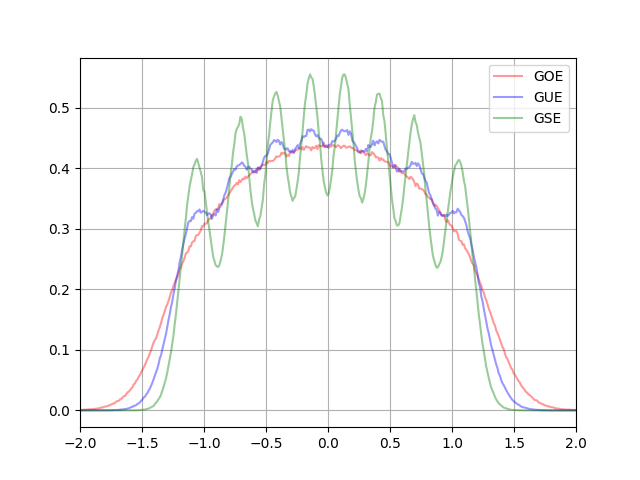
\includegraphics[width=0.8\linewidth]{FullGaussianDensityEscaled.png}
	\label{fig: lambdadist}
\end{center}

Mais desenvolvimento sobre a forma desta distribuição e as diferenças será feito posteriormente. Usaremos a referência \cite{Livan_2018} para a maior parte dos desenvolvimentos. Algum material interessante pode ser consultado em um livro de física em \cite{MEHTA1967v}.

\section{Física e Mecânica Estatística}
Estaremos lidando o tempo todo no nosso estudo com funções partições, de alguma forma, compartilhada com a física. Entenderemos um pouco mais sobre os desenvolvimentos do ensemble canônico na termodinâmica.


\subsection{Uma abordagem mais física}

Para o desenvolvimento da função partição estamos atentos aos requisitos do ensemble canônico. Um sistema termalizado por um banho térmico. Nosso sistema completo pode ser representado

\begin{center}
	\begin{tikzpicture}
		\fill[blue!10!white] (0,0) rectangle (8,3);
		\draw (0,0) rectangle (8,3);
		\fill[green!10!white] (0,0) rectangle (2,3);
		\draw (0,0) rectangle (2,3);
		\node at (1,2) {$\mathcal{S}$};
		\node at (1,0.5) {$E$};
		\node at (5,2) {$\mathcal{S}_r$};
		\node at (7.5,0.5) {$T$};
		\node at (3,0.5) {$E_t - E$};
	\end{tikzpicture}
\end{center}

Considere que os sistemas estão em contato térmico e o sistema completo, junto com o banho é um sistema isolado de energia $E_t$. Sabemos que a probabilidade de uma energia no nosso sistema termalizado ($\rho_E$) é expressa:

\[
	\rho_E = \sum_{\sigma} \rho_\sigma = \Omega(E)\rho_\sigma
\]

Onde note, $\rho_\sigma$ é a probabilidade de, dada uma temperatura, um microestado possível. Note por outro lado que podemos expressar:

\[
	\rho_E = \frac{\Omega(E) \Omega_r (E_t - E)}{\sum_{i} \Omega(E_i) \Omega_r(E_t-E)}
\]

Note que isso é nada mais do que dizer que os microestados são equiprováveis e basta uma contagem (normalizada) para definir a probabilidade. Neste sentido podemos também escrever:

\[
	\rho_\sigma \propto \Omega_r(E_t - E)
\]

Isso é, quanto mais formas o reservatório possa se organizar para determinada energia, mais provável é o microestado associado à energia de $\mathcal{S}$.

\begin{align*}
	\rho_\sigma & \propto e^{\beta T K_b \log{(\Omega_r(E_t - E))}} \\
				& \propto e^{\beta T \left( \mathcal{S}_r(E_t) - \frac{E}{T}\right) } \\
				& \propto e^{-\beta E} e^{\beta T \mathcal{S}_r(E_t)} \\
				& \propto e^{-\beta E}
\end{align*}

Onde fizemos a expansão de $k_b \log{(\Omega_r(E_t - E))}$ (entropia) em Taylor (apesar de que, em realidade, apenas $\frac{E}{E_t}$ é pequeno, não necessariamente $E$) e obtemos

\[
	\mathcal{S}_r(E_t - E) \approx \mathcal{S}_r(E_t) + \left( \frac{\partial \mathcal{S}_r}{\partial E}\right)_{E=E_t} (-E)
\]

Onde 

\[
	\left( \frac{\partial \mathcal{S}_r}{\partial E} \right)_{E=E_t} = \frac{1}{T}
\]

\subsection{A entropia de Shannon}

Podemos fazer algo um pouco mais matemático. Definiremos a entropia de Shannon

\[
	\mathcal{S} = -k_b \sum_{i} p_i \log{p_i}
\]

\subsubsection{Um vínculo}

Se impormos um vínculo do tipo

\[
	\sum_{i} p_i = 1
\]

Podemos usar os multiplicadores de Lagrange para realizar a maximização da nossa função. Pela definição, escrevemos:

\[
	S({p_i}, \lambda) \equiv k_b \sum_{i=1}^{N} p_i \log{(p_i)} - \lambda \left( \sum_{i=1}^{N}p_i -1 \right) 
\]

Com diferencial

\[
	\delta S = - k_b \sum_{i=1}^{N} \left( p_i \log{p_i} + \frac{p_i}{p_i} \delta p_i \right) - \lambda \sum_{i=1}^{N}\delta p_i
\]

Resolveremos agora o sistema

\[
 \begin{cases}
	\delta S = 0 \\
	\sum_{i} p_i = 1
\end{cases}
\]

ou seja,

\[
\begin{cases}
	-k_b (\log{p_i} + 1) - \lambda \\
	\sum_{i} p_i = 1
\end{cases}
\]

Note que $p_i = cte \ \forall i$. Teremos então $p_i = \frac{1}{N}$. A entropia neste caso será 

\[
	S({p_i}^*) = - k_b \sum_{i=1}^{N} \left( \frac{1}{N} \log{\frac{1}{N}} \right) = k_b \log{N}
\]

\subsubsection{Dois vínculos}

Faremos agora a implicação de um novo vínculo

\[
\sum_{\sigma} p_\sigma E_\sigma = U
\]

Desenvolvendo a equação

\[
S({p_i}, \lambda) \equiv k_b \sum_{i=1}^{N} p_i \log{(p_i)} - \lambda_1 \left( \sum_{i=1}^{N}p_i -1 \right)  - \lambda_2 \left( \sum_\sigma  p_\sigma E_\sigma - U \right) 
\]

Chegaremos no sistema


\[
\begin{cases}
	-k_b (\log{p_i} + 1) - \lambda_1 - \lambda_2 E_\sigma \\
	\sum_{\sigma} p_i = 1 \\
	\sum_{\sigma} p_\sigma E_\sigma = U
\end{cases}
\]

E finalmente, da primeira equação tiramos

\[
	p_\sigma = e^{A E_\sigma + B} = M e^{-\beta E_\sigma}
\]

De forma que podemos reescrever

\[
	1 = \sum_\sigma M e^{-\beta E_\sigma} = M \sum_\sigma e^{-\beta E_\sigma}
\]

Onde nomearemos $M = \frac{1}{\sum_{\sigma}e^{-\beta E_\sigma}} = \frac{1}{\mathcal{Z}}$ \textbf{função partição}. Falta apenas definir $\beta$ em

\[
	p_\sigma = \frac{e^{-\beta E_\sigma}}{Z}
\]

Para $\beta$ podemos aplicar o último vínculo (da temperatura térmica)

\[
	U = \sum_\sigma p_\sigma E_\sigma = \sum_\sigma \left( \frac{1}{Z} e^{-\beta E_\sigma} \right) E_\sigma = \frac{1}{Z} \sum_\sigma E_\sigma e^{-\beta E_\sigma}
\]

\[
	-\frac{1}{Z} \frac{\partial }{ \partial \beta} \left( \sum_\sigma e^{-\beta E_\sigma} \right) = -\frac{1}{\mathcal{Z}} \frac{\partial Z}{\partial \beta} = - \frac{\partial (\log{Z})}{\partial \beta}
\]

De alguma forma esta equação transcendental nos define $\beta$.

\subsection{Conexão Micro-Macro}

Quando tratamos destes sistemas no ensemble canônico a energia interna não mais será minimizada no nosso sistema termalizado. Introduzimos uma nova grandeza chamada Energia Livre de Helmholtz ($F$), definida como a transformada de Legendre (discutida no Apêndice \ref{apdx: legendre}) da energia interna em relação à entropia, ou seja

\begin{equation}
	 U(S,V,N) \mapsto F(T, V, N)
\end{equation}

ou ainda mais especificamente

\[
	F(T, V, N) = U(S(T,V,N), V, N) - T S(T,V,N) 
\]

Note ainda as diferenciais

\begin{align*}
	& dU = TdS - PdV + \mu dN \\
	& dF = -SdT - PdV + \mu dN
\end{align*}

Um sistema termalizado vai querer minimizar essa nova grandeza da energia livre de Helmholtz. Em todo caso iniciaremos com a expressão já deduzida da euqação de partição

\[
	\mathcal{Z} = \sum_{\sigma} e^{-\beta E_\sigma}
\]

Que pode ser reescrito em termos de uma soma na energia

\begin{align*}
	& \mathcal{Z} = \sum_{E} e^{-\beta E} \Omega(E) \\
	& \mathcal{Z} = \sum_{E} e^{-\beta T K_b \log{(\Omega(E))}} \Omega(E)
\end{align*}

Podemos argumentar que $ K_b \log{(\Omega(E))} = S(E)$ e usaremos o logaritmo de somas assintóticas (discutido no Apêndice \ref{apdx: somaassin}) para terminar o desenvolvimento. Note

\begin{align*}
	& \log{(\mathcal{Z})} \approx \log{\left( \max_x{[e^{-\beta(E - T S(E))}]} \right)} \\
	& \log{(\mathcal{Z})} \approx \log{\left(e^{-\beta \min_E{((E - T S(E)))}} \right)}
\end{align*}

Onde podemos reconhecer pela transformada de Legendre o termo referente à Energia livre de Helmholtz. Tendo assim

\[
	\log{(\mathcal{Z})} \approx -\beta F
\]	

\begin{equation}
	F = - K_b T \log{(\mathcal{Z})}
\end{equation}


\subsection{Entropia de Shannon}
Podemos fazer algo um pouco mais matemático. Definiremos a entropia de Shannon, que dá origem às expressões entrópicas gerais para qualquer ensemble.

\[
\mathcal{S} = -k_b \sum_{i} p_i \log{p_i}
\]

\subsubsection{Um vínculo}

Se impormos um vínculo do tipo

\[
\sum_{i} p_i = 1
\]

Podemos usar os multiplicadores de Lagrange para realizar a maximização da nossa função. Pela definição, escrevemos:

\[
S({p_i}, \lambda) \equiv k_b \sum_{i=1}^{N} p_i \log{(p_i)} - \lambda \left( \sum_{i=1}^{N}p_i -1 \right) 
\]

Com diferencial

\[
\delta S = - k_b \sum_{i=1}^{N} \left( p_i \log{p_i} + \frac{p_i}{p_i} \delta p_i \right) - \lambda \sum_{i=1}^{N}\delta p_i
\]

Resolveremos agora o sistema

\[
\begin{cases}
	\delta S = 0 \\
	\sum_{i} p_i = 1
\end{cases}
\]

ou seja,

\[
\begin{cases}
	-k_b (\log{p_i} + 1) - \lambda \\
	\sum_{i} p_i = 1
\end{cases}
\]

Note que $p_i = cte \ \forall i$. Teremos então $p_i = \frac{1}{N}$. A entropia neste caso será 

\[
S({p_i}^*) = - k_b \sum_{i=1}^{N} \left( \frac{1}{N} \log{\frac{1}{N}} \right) = k_b \log{N}
\]

\subsubsection{Dois vínculos}

Faremos agora a implicação de um novo vínculo

\[
\sum_{\sigma} p_\sigma E_\sigma = U
\]

Desenvolvendo a equação

\[
S({p_i}, \lambda_1, \lambda_2) \equiv k_b \sum_{i=1}^{N} p_i \log{(p_i)} - \lambda_1 \left( \sum_{i=1}^{N}p_i -1 \right)  - \lambda_2 \left( \sum_\sigma  p_\sigma E_\sigma - U \right) 
\]

Chegaremos no sistema


\[
\begin{cases}
	-k_b (\log{p_i} + 1) - \lambda_1 - \lambda_2 E_\sigma  = 0\\
	\sum_{\sigma} p_i = 1 \\
	\sum_{\sigma} p_\sigma E_\sigma = U
\end{cases}
\]

E finalmente, da primeira equação tiramos

\[
p_\sigma = e^{A E_\sigma + B} = M e^{-\beta E_\sigma}
\]

De forma que podemos reescrever

\[
1 = \sum_\sigma M e^{-\beta E_\sigma} = M \sum_\sigma e^{-\beta E_\sigma}
\]

Onde nomearemos $M = \frac{1}{\sum_{\sigma}e^{-\beta E_\sigma}} = \frac{1}{\mathcal{Z}}$ \textbf{função partição}. Falta apenas definir $\beta$ em

\[
p_\sigma = \frac{e^{-\beta E_\sigma}}{Z}
\]

Para $\beta$ podemos aplicar o último vínculo (da temperatura térmica)

\[
U = \sum_\sigma p_\sigma E_\sigma = \sum_\sigma \left( \frac{1}{Z} e^{-\beta E_\sigma} \right) E_\sigma = \frac{1}{Z} \sum_\sigma E_\sigma e^{-\beta E_\sigma}
\]

\[
-\frac{1}{Z} \frac{\partial }{ \partial \beta} \left( \sum_\sigma e^{-\beta E_\sigma} \right) = -\frac{1}{\mathcal{Z}} \frac{\partial Z}{\partial \beta} = - \frac{\partial (\log{Z})}{\partial \beta}
\]

De alguma forma esta equação transcendental nos define $\beta$.

\subsubsection{Três vínculos}

Introduziremos um terceiro novo vínculo

\[
	\sum_\sigma p_\sigma N_\sigma = N
\]

Da mesma forma, teremos que desenvolver a equação

\[
S({p_i}, \lambda_1, \lambda_2, \lambda_3) \equiv k_b \sum_{i=1}^{N} p_i \log{(p_i)} - \lambda_1 \left( \sum_{i=1}^{N}p_i -1 \right)  - \lambda_2 \left( \sum_\sigma  p_\sigma E_\sigma - U \right) - \lambda_3 \left( \sum_\sigma  p_\sigma N_\sigma - N \right) 
\]

Do sistema associado aos vínculos de Lagrange

\[
\begin{cases}
	-k_b (\log{p_i} + 1) - \lambda_1 - \lambda_2 E_\sigma  - \lambda_3 N_\sigma = 0\\
	\sum_{\sigma} p_i = 1 \\
	\sum_{\sigma} p_\sigma E_\sigma = U \\
	\sum_{\sigma} p_\sigma N_\sigma = N
\end{cases}
\]

Da primeira equação tiramos

\[
p_\sigma = e^{A E_\sigma + B N_\sigma + C} = M e^{-\beta E_\sigma +\beta \mu N_\sigma}
\]

De forma que podemos reescrever

\[
1 = \sum_\sigma M e^{-\beta E_\sigma +\beta \mu N_\sigma} = M \sum_\sigma e^{-\beta E_\sigma +\beta \mu N_\sigma}
\]

Novamente nomearemos $Z$ em 

\[
	M = \frac{1}{\sum_\sigma e^{-\beta E_\sigma +\beta \mu N_\sigma}} = \frac{1}{Z}
\]

a função partição. As outras duas equações nos definem $\beta$ e $\mu$.

\subsection{O ensemble Micro-Canônico}
O ensemble Micro-Canônico devera ser o mais simples que desenvolveremos. Para este caso a energia é constante e todo microestados devem ser igualmente prováveis pela hipótese ergótica.

\begin{center}
	\begin{tikzpicture}
		\fill[green!10!white] (0,0) rectangle (2,3);
		\draw (0,0) rectangle (2,3);
		\node at (1,2) {$\mathcal{S}$};
		\node at (1,0.5) {$E$};
	\end{tikzpicture}
\end{center}

Sabemos então que vamos querer minimizar a entropia usual com

\begin{equation}
	U(S,V,N)  
\end{equation}

Com 

\[
	dU = TdS - PdV + \mu N
\]

e, especialmente

\[
\rho_E = \sum_{\sigma} \rho_\sigma = \Omega(E) \rho_\sigma
\]

Ou ainda, se $\Omega(E)$ é a quantidade de microestados,

\[
	 \rho_\sigma = \frac{1}{\Omega(E)}
\]

De forma que nossa função partição será

\[
	Z = \sum_\sigma \frac{1}{\Omega(E)} = 1
\]

E em relação a energia

\[
	Z = \sum_E \frac{1}{\Omega(E)} \Omega(E) = \exp{\left\lbrace \beta T k_b \log{\frac{1}{\Omega(E)}} \right\rbrace } \Omega(E) 
\]

Finalmente

\[
 \log{(Z)} = 0 = -\frac{S}{k_b} + \log(\Omega(E))
\]

Ou melhor

\begin{equation}
	S = k_b \log{(\Omega(E))}
\end{equation}

\subsection{O ensemble Canônico}
Quando tratamos destes sistemas no ensemble canônico a energia interna não mais será minimizada no nosso sistema termalizado. Introduzimos uma nova grandeza chamada Energia Livre de Helmholtz ($F$), definida como a transformada de Legendre (discutida no Apêndice \ref{apdx: legendre}) da energia interna em relação à entropia, ou seja

\begin{equation}
	U(S,V,N) \mapsto F(T, V, N)
\end{equation}

ou ainda mais especificamente

\[
F(T, V, N) = U(S(T,V,N), V, N) - T S(T,V,N) 
\]

Note ainda as diferenciais

\begin{align*}
	& dU = TdS - PdV + \mu dN \\
	& dF = -SdT - PdV + \mu dN
\end{align*}

Para o desenvolvimento da função partição estamos atentos aos requisitos do ensemble canônico. Um sistema termalizado por um banho térmico. Nosso sistema completo pode ser representado

\begin{center}
	\begin{tikzpicture}
		\fill[blue!10!white] (0,0) rectangle (8,3);
		\draw (0,0) rectangle (8,3);
		\fill[green!10!white] (0,0) rectangle (2,3);
		\draw (0,0) rectangle (2,3);
		\node at (1,2) {$\mathcal{S}$};
		\node at (1,0.5) {$E$};
		\node at (5,2) {$\mathcal{S}_r$};
		\node at (7.5,0.5) {$T$};
		\node at (3,0.5) {$E_t - E$};
	\end{tikzpicture}
\end{center}

Considere que os sistemas estão em contato térmico e o sistema completo, junto com o banho é um sistema isolado de energia $E_t$. Sabemos que a probabilidade de uma energia no nosso sistema termalizado ($\rho_E$) é expressa:

\[
\rho_E = \sum_{\sigma} \rho_\sigma = \Omega(E)\rho_\sigma
\]

Onde note, $\rho_\sigma$ é a probabilidade de, dada uma temperatura, um microestado possível. Note por outro lado que podemos expressar:

\[
\rho_E = \frac{\Omega(E) \Omega_r (E_t - E)}{\sum_{i} \Omega(E_i) \Omega_r(E_t-E)}
\]

Note que isso é nada mais do que dizer que os microestados são equiprováveis e basta uma contagem (normalizada) para definir a probabilidade. Neste sentido podemos também escrever:

\[
\rho_\sigma \propto \Omega_r(E_t - E)
\]

Isso é, quanto mais formas o reservatório possa se organizar para determinada energia, mais provável é o microestado associado à energia de $\mathcal{S}$.

\begin{align*}
	\rho_\sigma & \propto e^{\beta T K_b \log{(\Omega_r(E_t - E))}} \\
	& \propto e^{\beta T \left( \mathcal{S}_r(E_t) - \frac{E}{T}\right) } \\
	& \propto e^{-\beta E} e^{\beta T \mathcal{S}_r(E_t)} \\
	& \propto e^{-\beta E}
\end{align*}

Onde fizemos a expansão de $k_b \log{(\Omega_r(E_t - E))}$ (entropia) em Taylor (apesar de que, em realidade, apenas $\frac{E}{E_t}$ é pequeno, não necessariamente $E$) e obtivemos

\[
\mathcal{S}_r(E_t - E) \approx \mathcal{S}_r(E_t) + \left( \frac{\partial \mathcal{S}_r}{\partial E}\right)_{E=E_t} (-E)
\]

Onde 

\[
\left( \frac{\partial \mathcal{S}_r}{\partial E} \right)_{E=E_t} = \frac{1}{T}
\]

Um sistema termalizado vai querer minimizar essa nova grandeza da energia livre de Helmholtz. Em todo caso iniciaremos com a expressão já deduzida da equação de partição

\[
\mathcal{Z} = \sum_{\sigma} e^{-\beta E_\sigma}
\]

Que pode ser reescrito em termos de uma soma na energia

\begin{align*}
	& \mathcal{Z} = \sum_{E} e^{-\beta E} \Omega(E) \\
	& \mathcal{Z} = \sum_{E} e^{-\beta T K_b \log{(\Omega(E))}} \Omega(E)
\end{align*}

Podemos argumentar que $ K_b \log{(\Omega(E))} = S(E)$ e usaremos o logaritmo de somas assintóticas (discutido no Apêndice \ref{apdx: somaassin}) para terminar o desenvolvimento. Note

\begin{align*}
	& \log{(\mathcal{Z})} \approx \log{\left( \max_x{[e^{-\beta(E - T S(E))}]} \right)} \\
	& \log{(\mathcal{Z})} \approx \log{\left(e^{-\beta \min_E{((E - T S(E)))}} \right)}
\end{align*}

Onde podemos reconhecer pela transformada de Legendre o termo referente à Energia livre de Helmholtz. Tendo assim

\[
\log{(\mathcal{Z})} \approx -\beta F
\]	

\begin{equation}
	F = - K_b T \log{(\mathcal{Z})}
\end{equation}


\subsection{O ensemble Grão Canônico}
Supomos agora nosso sistema novamente controlado por um banho térmico. Desta vez permitiremos a troca de temperatura e partículas. Definiremos uma energia livre tal que $U(S,V,N) \mapsto \Phi(T,V,\mu)$. Chamaremos esta energia livre de Grão Potencial ou Potencial de Landau. Como sempre, definiremos o potencial como uma transformada de Legendre sob a Energia

\begin{equation}
	\Phi = U - TS - \mu N
\end{equation}

\[
	\Phi(T,V,\mu) = U(S(T,V,\mu), V, N(T,V,\mu)) - TS(T,V,\mu) - \mu N(T,V,\mu)
\]

e é claro, na diferencial

\[
	d\Phi = dU - Tds - SdT - \mu dN - Nd\mu
\]

Onde lembramos que $d\Phi = TdS - PdV + \mu dN$ de forma que

\[
	d\Phi = -SdT - PdV - Nd\mu
\]

Ou seja,

\[
	S = - \left| \frac{\partial \Phi}{\partial T} \right|_{V,N} 
\]
\[
	N = - \left| \frac{\partial \Phi}{\partial \mu} \right|_{T,V} 
\]

Tratamos do seguinte sistema,

\begin{center}
	\begin{tikzpicture}
		\fill[blue!10!white] (0,0) rectangle (8,3);
		\fill[green!10!white] (0,0) rectangle (2,3);
		\draw (0,0) rectangle (8,3);
		\draw[dashed] (2,0) -- (2,3);
		\node at (1,2) {$\mathcal{S}$};
		\node at (1,0.5) {$E,N$};
		\node at (5,2) {$\mathcal{S}_r$};
		\node at (7.5,0.5) {$T,\mu$};
		\node at (3,0.7) {$E_t - E$};
		\node at (3,0.3) {$N_t - N$};
	\end{tikzpicture}
\end{center}

Sabemos afirmar que $p_{\sigma} \propto \Omega_R (E_t - E, N_t - N)$, ou seja, cada microestado do nosso sistema é proporcional às formas que o banho pode se arranjar dado $(E,N)$. Ou seja

\begin{align*}
	p_{\sigma} & = \exp{ \lbrace \log{[\Omega_R(E_t - E, N_t - N)]} } \rbrace \\
	& \propto exp{\left\lbrace \frac{1}{k_b} \left[  k_b \log{(\Omega_R(E_T, N_T))} - E \frac{\partial}{\partial E'} (k_b log{\Omega_R(E', N')})\middle|_{N'=N_T}^{E'=E_T} -  N \frac{\partial}{\partial N'} (k_b log{\Omega_R(E', N')})\middle|_{N'=N_T}^{E'=E_T} \right]  \right\rbrace} \\
	& \propto \exp{\left\lbrace  \frac{1}{k_b} \left[  - E \frac{\partial}{\partial E'} (k_b log{\Omega_R(E', N')})\middle|_{N'=N_T}^{E'=E_T} -  N \frac{\partial}{\partial N'} (k_b log{\Omega_R(E', N')})\middle|_{N'=N_T}^{E'=E_T} \right] \right\rbrace}
\end{align*}

Onde retiramos o termo que não depende do nosso sistema de interesse e será constante, agregando ele na proporcionalidade. Agora faremos uso da ideia da entropia como $S = k_b \log{(\Omega_R(E',N'))}$ para escrever a relação acima em termos da temperatura e potencial químico. Usando das derivadas parciais da entropia em $dS = \frac{1}{T} dU + \frac{P}{T} dV - \frac{\mu}{T} dN$,

\begin{align*}
	p_{\sigma} & \propto \exp{\left\lbrace  \frac{1}{k_b} \left[  -E \frac{1}{T} - N \frac{\mu}{T} \right]  \right\rbrace} \\
	& \propto e^{-\beta E + \beta \mu N}
\end{align*}

e

\begin{equation}
	p_\sigma = \frac{1}{\Xi} e^{-\beta E + \beta \mu N}
\end{equation}

Onde 

\begin{equation}
	\Xi = \sum_\sigma e^{-\beta E + \beta \mu N}
\end{equation}

O log da nossa função partição deve resultar em uma expressão de energia livre.

\begin{align*}
	\log{\Xi} & = \log{ \left( \sum_\sigma e^{-\beta E_\sigma + \beta \mu N_\sigma} \right) } \\
	& = \log{ \left( \sum_{E,N}  \Omega(E,N) e^{-\beta E + \beta \mu N} \right) } \\
	& = \log{ \left( \sum_{E,N}  \exp{\left\lbrace \frac{k_b}{k_b} \log{\Omega(E,N)}\right\rbrace}  \exp{\left\lbrace (-\beta E + \beta N \mu) \right\rbrace} \right) } \\
	& = \log{ \left( \sum_{E,N}  \exp{\left\lbrace \frac{T}{k_b T} S - \beta E + \beta N \mu \right\rbrace} \right) } \\
	& = \log{ \left( \sum_{E,N}  e^{ \beta(E - TS - N \mu)} \right) } \\
\end{align*}

Para a aproximação desta expressão vamos considerar que o logaritmo de uma somatória pode ser aproximada por seu termo máximo,

\[
	\approx \log{ e^{ \beta(E^* - TS(E^*,N^*) - N^* \mu)}} = \beta(E^* - TS(E^*,N^*) - N^* \mu)
\]

Ou seja,

\[
\log{\Xi} = \beta(E^* - TS(E^*,N^*) - N^* \mu) = -\beta \Phi
\]

e finalmente,

\begin{equation}
	\Phi = -k_b T \log{\Xi}
\end{equation}

\chapter{Procura-se autovalores}
A distribuição dos autovalores de uma matriz aleatória Gaussiana $N\times N$ é dada por:

\begin{equation}
	\rho(\mmany{x}{N}) = \frac{1}{\mathcal{Z}_{N,\beta}} e^{-\frac{1}{2} \sum_{i=1}^{N} x_i^2} \prod_{j<k} |x_j - x_k|^{\beta}
	\label{eq: dist geral gaussiana}
\end{equation}

onde a constante de normalização $\mathcal{Z}$ é dada por

\begin{equation}
		\mathcal{Z}_{N, \beta} = (2\pi)^{\frac{N}{2}} \prod_{j=1}^{N} \frac{\Gamma (1 + j \frac{\beta}{2})}{\Gamma (1 + \frac{\beta}{2})}
\end{equation}

$\beta$ é o index de Dyson e indica o ensemble que utilizamos. Mais importante é notar que existe na nossa distribuição um fator de repulsão e um fator de campo de mínimo de energia em $x=0$. De forma que mesmo centradas em $0$ as partículas mantém uma distância entre si pela repulsão 'Coulombiana'.

Se quisermos computar o histograma dos autovalores podemos tomar a marginal

\begin{equation}
	\rho(x) = \int \cdots \int \mcmany{dx}{N}{\cdot} \rho(x, x_2, \cdots, x_N)
\end{equation}

Ou seja, o perfil da função partição de uma nova partícula dada o posicionamento das outras. Para a Equação \ref{eq: dist geral gaussiana}, a densidade espectral $\mathbb{E}[n(x)]=\rho(x)$ é dada pelo limite

\begin{equation}
	\lim_{N \rightarrow \infty} \sqrt{\beta N} \rho(\sqrt{\beta N} x) = \rho_{sc}(x)
\end{equation}

Onde $\rho_{sc}(x) = \frac{1}{\pi} \sqrt{2 - x^2}$ compõe a famosa lei do semi-círculo de Wigner representada na Figura \ref{fig: lambdadist}. Os pontos $\pm \sqrt{2 \beta N}$ são as bordas espectrais. Um esquema útil para organização dos multiplos ensembles é a classificação de Layman. Denomina-se

\begin{enumerate}
	\item \textbf{Entradas Independentes}: Adicionada a necessidade de simetria, matrizes deste tipo são chamadas matrizes de Wigner.
	\item \textbf{Invariantes por rotação}: Quaisquer duas matrizes que são relacionadas por uma transformação $\matriz{H'} = \matriz{U} \matriz{H} \matriz{U}^{-1}$ ocorrerão com a mesma probabilidade.
\end{enumerate}

Só existe um tipo especial de matriz que se encontra na intersecção e são as classes Gaussianas.

Em geral no mundo das matrizes aleatórias três classes são muito importantes e serão atores centrais no nosso estudo. São as três classes associadas às matrizes que tem entradas gaussianas. Estas são: O Ensemble Gaussiano Ortogonal (GOE), O Ensemble Gaussiano Unitário (GUE) e o Ensemble Gaussiano Simplético (GSE). Em suma, eles tratam, em ordem, de matrizes com entradas gaussianas reais, complexas e quaterniônicas. Seus nomes estão relacionados com a matriz necessária para a transformação de diagonalização das matrizes. Unitária para o caso complexo, por exemplo. Seus autovalores possuem distribuições distintas (ao menos para a escala usada) e é ilustrada abaixo na Figura \eqref{fig: lambdadist}.

\begin{center}
	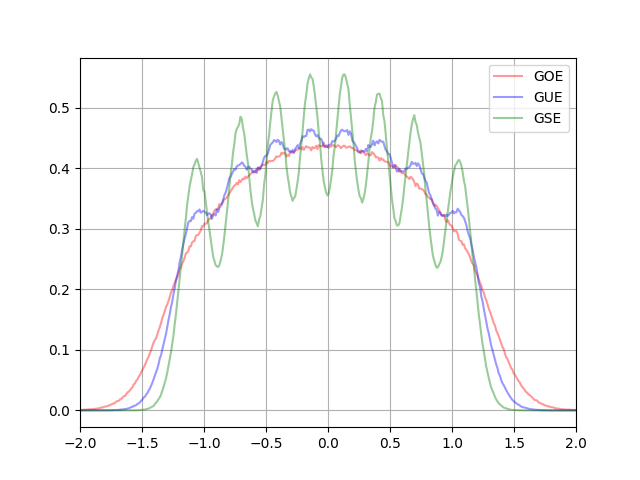
\includegraphics[width=0.8\linewidth]{FullGaussianDensityEscaled.png}
	\label{fig: lambdadist}
\end{center}

Mais desenvolvimento sobre a forma desta distribuição e as diferenças será feito posteriormente. Usaremos a referência \cite{Livan_2018} para a maior parte dos desenvolvimentos. Algum material interessante pode ser consultado em um livro de física em \cite{MEHTA1967v}.

\section{Porquê exponencial?}
\subsection{Shannon-Quem?}

O uso da p.d.f gaussiana pode ser justificado de algumas formas. Uma primeira abordagem a ser explorada é a de maximização entrópica ou minimização de informação similar aos trabalhos de Shannon-Kinchin. Definiremos uma grandeza $\mathcal{I}[\mathcal{P}(\matriz{H})]$ associada à uma p.d.f tal que:

\[
	\mathcal{I}[\mathcal{P}(\matriz{H})] = - \int d\mu (\matriz{H}) \mathcal{P}(\matriz{H}) \ln{\mathcal{P}(\matriz{H})} 		
\]

Que é uma extensão natural da definição discreta de informação $- \sum_{l=1}^{m} p_m \ln{p_m}$. Agora argumentaremos algo parecido com os argumentos usados em termodinâmica de maximização de entropia. Diremos que a incerteza sobre as matrizes será máxima, ou seja, teremos a maior aleatoriedade das matrizes quando a entropia for maximizada e a informação, minimizada. Assim como na entropia física impomos um vínculo de energia constante, aqui faremos algo do tipo $E(\Tr{\matriz{H}}) = b$ e $E((\Tr{\matriz{H}})^2) = a > 0$. Vamos introduzir esses vinculos como multiplicadores de lagrange com multiplicadores $v_1$ e $v_2$. 

\[
	\mathcal{I}[\mathcal{P}(\matriz{H})] = - \int d\mu (\matriz{H}) \mathcal{P}(\matriz{H}) \left( \ln{\mathcal{P}(\matriz{H})} - v_1 \Tr{\matriz{H}} - v_2 \Tr{\matriz{H}}^2 \right)	
\]	

que tem diferencial

\[
\delta \mathcal{I}[\mathcal{P}(\matriz{H})] = - \int d\mu (\matriz{H})  \delta \mathcal{P}(\matriz{H}) \left( 1 + \ln{\mathcal{P}(\matriz{H})} - v_1 \Tr{\matriz{H}} - v_2 \Tr{\matriz{H}}^2 \right)	= 0
\]

Que só vai ser mínimo se 

\[
	\mathcal{P}(\matriz{H}) \propto e^{ - v_1 \Tr{\matriz{H}} - v_2 \Tr{\matriz{H}}^2}
\]

Onde os multiplicadores são unicamente definidos pelas constantes do vínculo. Esse fato motiva de alguma forma o estudo da p.d.f gaussiana para as matrizes.

\section{Independência ou Morte}
Consideremos matrizes com entradas independentes. Qual a função densidade de probabilidade (F.P.D.) da matriz simétrica $\matriz{H_s}$? Devemos fazer separadamente a diagonal da seção triangular que formos usar e teremos

\[
\rho((\matriz{H_s})_{11}, \dots, (\matriz{H_s})_{NN}) = \prod_{i=1}^{N} \left[ \frac{e^{\frac{-(H_s)^2_{ii}}{2}}}{2\pi} \right] \prod_{i<j} \left[ \frac{e^{-(H_s)^2_{ij}}}{\sqrt{\pi}} \right]
\]

Podemos também definir a distribuição para os autovalores de uma matriz Gaussiana de dimensão $N$ como \footnote{Esse resultado é não óbvio e deve ser discutido em breve.}

\begin{equation}
	\rho(x_1, \dots, x_N) = \frac{1}{\mathcal{Z_{N, \beta}}} e^{-\frac{1}{2} \sum_{i=1}^{N} x_i^2} \prod_{j<k} | x_j - x_k |^{\beta}
\end{equation}

onde a constante de normalização é dada por

\[
\mathcal{Z_{N, \beta}} = (2\pi)^\frac{N}{2} \prod_{j=1}^{N} \frac{\Gamma(1+ j\frac{\beta}{2})}{\Gamma(1+ \frac{\beta}{2})}
\]

Para ressaltar um pouco do jargão, $\beta$ é denominado \textit{Dyson Index} que em suma se refere à "dimensão" das suas entradas na matriz. $1$ para GOE, $2$ para GUE e $4$ para GSE.

Algumas observações sobre essa expressão são interessantes. Note que o fator exponencial deve matar qualquer chance de uma matriz com autovalor alto. Ao mesmo tempo o fator de dependência deve matar qualquer configuração com autovalores muito próximos entre si. Existe um efeito de repelência entre autovalores na expressão.

\section{Uma medida à Hermitiana}
Consideraremos no nosso estudo para referencia matrizes quadradas de entradas complexas com dimensão $N$. Nosso objetivo é afinal ter uma forma de mensurar a distribuição de autovalores e para isso, faremos os seguintes desenvolvimentos.

Consideremos inicialmente um espaço de matrizes com entradas complexas $2N^2$ dimensional. Contido neste espaço temos um espaço de maior interesse correspondente ao espaço das matrizes \textit{hermitianas} de dimensão $N^2$. A escolha do subespaço está relacionada com o fato que matrizes hermitianas são diagonalizáveis e a distribuição de seus autovalores estará diretamente relacionada (com uma mudança de base) à distribuição do traço da matriz diagonalizada. Note que para a matriz diagonal ter a mesma medida que nossa matriz inicial, nossa medida deve ser invariável por rotação.

Mais detalhadamente podemos escrever nossa matriz hermitiana $\matriz{H}$ como 

\[
\matriz{H} = \matriz{U} \matriz{\Lambda} \matriz{U}^{-1} \ , \ \matriz{\Lambda} = diag(\lambda_1, \dots, \lambda_2) \ , \ \matriz{U}\cdot\matriz{U}^* = I
\]

onde, claro, $\matriz{\Lambda}$ é diagonal de autovalores e $\matriz{U}$ é unitária e com colunas equivalentes aos autovetores de $\matriz{H}$. Em geral, o conjunto de matrizes degeneradas tem medida nula e não é uma preocupação. Um cuidado deve ser tomado. A correspondência $\matriz{H} \implies (\matriz{U} \ U(N), \matriz{\Lambda})$ não é injetora, podemos tomar $\matriz{U}_1 \matriz{\Lambda} \matriz{U}_1^{-1} = \matriz{U}_2 \matriz{\Lambda} \matriz{U}_2^{-1}$ se $\matriz{U}_1^{-1} \matriz{U}_2 = diag(e^i\phi_1, \dots, e^i\phi_N)$ para qualquer escolha de fases $(\phi_1, \dots, \phi_N)$. Para restringir nosso problema e tornar a função injetiva será necessário considerar as matrizes unitárias ao espaço de coset $U(N) / U(1) \times \dots \times U(1)$ \footnote{Não tenho muita ideia de espaços de Coset. Pelo que entendo, existe um espaço onde toda $\matriz{U}$ pode ser representada por $\matriz{U}_c \matriz{U}_d$, onde $\matriz{U}_c$ compõe o espaço de coset e $\matriz{U}_d$ é uma matriz diagonal unitária. Dessa forma matrizes equivalentes são aquelas que multiplicadas por $\matriz{U}_d$ tem um mesmo resultado.}. Uma outra restrição necessárias é ordenas os autovalores, ou seja, $\lambda_1 < \dots < \lambda_n$. Temos que reescrever agora a medida $d\mu(\matriz{H})$ em função de auvalores e da $\matriz{U}$ de autovetores.

Para resumir o desenvolvimento, alguns resultados serão diretamente enunciados. Essa seção pode ser encontrada no relatório \cite{fyodorov2010introduction}. Em especial recuperaremos o elemento de distância e volume no subespaço que vamos tratar

\begin{equation}
	(ds)^2 = \Tr{d\matriz{H} d\matriz{H}^*} = \sum_{i} (dx_{ii})^2 + 2 \sum_{i < j} \left[(dx_{ij})^2 + (dy_{ij})^2 \right]
	\label{eq: ds}
\end{equation}

\begin{equation}
	d\mu(\matriz{H}) = 2^{\frac{N(N-1)}{2}} \prod_{i} dx_{ii} \prod_{i<j} dx_{ij} dy_{ij}
	\label{eq: du}
\end{equation}

Ambos vem de um desenvolvimento da métrica do espaço discutido. Note que nossa medida de comprimento é invariante em respeito à automorfismos. Especificamente, se tomarmos os elementos \eqref{eq: ds} e \eqref{eq: du} na decomposição espectral, obteremos

\begin{equation}
	(ds)^2 = \sum_{i} (d\lambda)^2 + \sum_{i<j} (\lambda_i - \lambda_j)^2 \overline{\delta U_{ij}} \delta U_{ij}
\end{equation}

e

\begin{equation}
	d\mu(\matriz{H}) = \prod_{i < j} (\lambda_i - \lambda_j)^2 \prod_{i} d\lambda_i \times d\mu(\matriz{U})
\end{equation}

Tendo a medida de integração pronta, podemos definir uma F.D.P $\mathcal{P}(\matriz{H})$ neste espaço de matizes hermitianas tal que $\mathcal{P}(\matriz{H}) d\mu(\matriz{H})$ é a probabilidade da matriz $\matriz{H}$  estar no volume $d\mu(\matriz{H})$. Queremos que nossa função seja invariante à rotação, ou seja, $\mathcal{P}(\matriz{H}) = \mathcal{P}( \matriz{U}^* \matriz{H} \matriz{U})$.

Conhecer os $N$ primeiros traços ($\Tr{\matriz{H}^n}$) de $\matriz{H}$ define unicamente o polinômio característico e junto com ele, os autovalores. Especificamente tomaremos 

\begin{equation}
	\mathcal{P}(\matriz{H}) = Ce^{-\Tr{Q(\matriz{H})}}
	\label{eq: p}
\end{equation}

Onde $Q$ deve ser um polinômio de até ordem $2j \leq N$ suficiente para garantir a convergência de

\[
	\mathcal{Z}_n = \int_{\mathcal{H}_n} e^{-\Tr{Q(\matriz{M})}} d\matriz{M} 
\]

Comumente uma condição suficiente é

\[
	\lim_{x \rightarrow \pm \infty} \frac{Q(x)}{\ln{(1+x^2)}} = \infty
\]

Mas em especial, se tomarmos

\[
	Q(x) = ax^2 + bx + c
\]


Nossa medida tomará a forma

\begin{align}	
	\mathcal{P}(\matriz{H}) & = e^{-a \left[ \sum_{i} x_{ii}^2 + 2 \sum_{i < j} [x_{ij}^2 + y_{ij}^2] \right] } e^{-b \sum_{i} x_{ii}} e^{-c N} \\
	& = e^{-cN} \prod_{i=1}^{N} \left( e^{-ax^2_{ii}-bx_{ii}} \right) \prod_{i<j} e^{-2ax^2_{ij}} \prod_{i<j} e^{-2ay^2_{ij}}
\end{align}

Onde podemos notar que a distribuição de probabilidade da matriz $\matriz{H}$ pode ser representados por fatores independentes, cada um de forma gaussiana. Para este potencial, temos uma conexão entre as matrizes de entrada independentes e as matrizes invariáveis por rotação. Lembre-se que para as variáveis serem independentes $\mathcal{P}$ deve ter a forma $\mathcal{P} = Ce^{-\left( a\Tr{\matriz{H}^2} + b\Tr{\matriz{H}} + cN \right)}$ para constantes $a>0, b, c$. Em nota, sabemos então

\[
e^{\Tr{V(\matriz{H})}}  d\mu(\matriz{H}) = e^{-\sum_{j} V(\lambda_j)}  \prod_{i < j} (\lambda_i - \lambda_j)^2 d\mu(\lambda) d\mu(\matriz{U})
\]

ou mais geralmente para o ensemble com 

\[
	\frac{1}{{\mathcal{\tilde{Z}}}_n} e^{\Tr{(V(\matriz{M}))}} dM
\]

Dado $\lambda_j$ os autovalores

\[
	\Tr{(V(\matriz{M}))} = -\sum_{j=1}^{n} V(\lambda_j)
\]

e finalmente podemos escrever

\begin{align}
	E[f]& = \int_{\mathcal{H}_n} f(\matriz{M}) e^{-\Tr{(Q(\matriz{M}))}} d\matriz{M} \\
	&  = \frac{1}{\mathcal{Z}} \int \dots \int f(\lambda_1, \dots, \lambda_n) \prod_{i < j} (\lambda_i - \lambda_j)^2 \prod_{j=1}^{n} e^{-Q(\lambda_j)} d\lambda_1 \dots d\lambda_n
\end{align}

Assim, a probabilidade conjunta nas matrizes induz uma densidade de probabilidade de autovalores

\[
	\frac{1}{\mathcal{Z}_n} \prod_{i<j} (\lambda_i - \lambda_j)^2 \prod_{j=1}^{n} e^{Q(\lambda_j)}
\]

Alguns resultados foram resgatadas da nota do autor em \cite{ArnoLectureNotes}.{\tiny }

\chapter{Movimento Browniano}
\input{chapters/brownian}

\section{Processo Pontual}
Um processo pontual pode ser interpretado como um conjunto aleatório de pontos ou como a medida de probabilidade associada a esse conjunto. Um processo pontual possui $n$ pontos se

\[
\mathcal{P}(\# X=n) = 1
\]

Onde $X$ é um conjunto enumerável de $\mathcal{X}$ ($\mathbb{R}$, $\mathbb{Z}$ ou um subconjunto destes). O conjunto de todas configurações possíveis é denominado $Conf(\mathcal{X})$. Se $P(x_1, \dots, x_n)$ é uma função de densidade de probabilidade em $\mathbb{R}^n$ invariante por permutações

\[
	\mathbb{R}^n \rightarrow Conf(\mathbb{R})
\]
\[
	(x_1, \dots, x_n) \mapsto X = {x_1, \dots, x_n}
\]

define naturalmente um processo pontual com $n$ pontos.

\subsection{Poisson \& fries}

Tome $\set{N(t)}$ o número de eventos no intervalo de tempo $]0,t]$. $\set{N(t)}$  é um processo estocástico (de contagem). Se o processo de Poisson possui $\lambda > 0$, para um elemento fiox do espaço amostral a variável aleatória $N$ assume valor $k$ no tempo $t$ com probabilidade

\begin{equation}
	\mathcal{P}[N(t) = k] = \frac{(\lambda t)^k e^{-\lambda t}}{k!}
\end{equation}

Onde $\lambda$ é o número esperado de chagadas por unidade de tempo. Agora, como um processo pontual, a probabilidade de n eventos no intervalo $]a,b]$ é

\[
	\mathcal{P}(N]a,b] = n) =  \frac{(\lambda (b-a))^n e^{-\lambda (b-a)}}{n!}
\]

Podemos usar a independência de cada evento de Poisson em intervalos disjuntos para escrever

\[
	\mathcal{P}(N]a_1,b_1] = n_1, \dots, N]a_k,b_k] = n_k) = \prod_{i=1}^{k} \frac{(\lambda (b_i-a_i))^n_i e^{-\lambda (b_i-a_i)}}{n_i!}
\]

Podemos escrever para uma função $f$ mensurável em $\mathbb{R}$

\[
	\sum_{x_i \in \mathcal{X}} f(x_i) = \int f(x) dN(x)
\]

Onde a medida dN é

\[
	dN(x) = \sum_{x_i \in \mathcal{X}} \delta_{x_i} (x)
\]

Onde notamos que podemos interpretar tanto quanto uma soma de um processo pontual quanto uma medida de probabilidade.


\subsection{Funcão Correlação}

Definimos uma variável aleatória $N$ anteriormente. Naturalmente, poderíamos estar interessados em sua esperança. Mais especificamente, podemos procurar a esperança do número de pontos de uma ocnfiguração dentro de um intervalo $A \subset \mathbb{R}$.

\[
	A \mapsto \mathbb{E}[N(A)] = \mathbb{E}[\#(A \cap X)]	
\]

Que pode ser interpretada como uma medida com densidade $p_1$

\begin{equation}
	\mathbb{E}[\#(A \cap X)] = \int_{A} p_1(x) dx
	\label{eq: p1}
\end{equation}

A equação \ref{eq: p1} é conhecida como \textit{função de correlação de 1 ponto}. Em grosso modo, $p_1(x)$ é a probabilidade de haver um ponto da configuração entre $x$ e $x+dx$. Seja um configuração simples $X = \set{x_1, \dots, x_n}$ e intervalos disjuntos na reta \many{A}{n},

\[
	\int_A \dots \int_A \rho_n(x_1, \dots, x_n) dx_1, \dots, dx_n = \mathbb{E} \left( \prod_{j=1}^{k} \# (X \cap A_j) \right) 
\]

é o número esperado de n-uplas (\many{x}{n}) $\in A_1 \times \dots \times A_n$ tais que $x_i \in A_i, i=1,\dots,n$. Seja $\mathbb{P}(x_1, \dots, x_n)$ uma densidade de probabilidade em $\mathbb{R}^n$, então o processo pontual de n pontos gerado possui funções de correlação dadas por

\[
	p_k(x_1, \dots, x_k) = \frac{n!}{(n-k)!} \int \dots \int \mathbb{P}(x_1, \dots, x_n) dx_{k+1}\dots dx_n
\]


\subsection{Pontual Determinantal}

Um processo pontual vai ser chamado determinantal se dada uma função de correlação $\rho_n$, existe um núcleo $K(x, y)$ conhecido como núcleo de correlação tal que

\begin{equation}
	\rho_n(x_1, \dots, x_n) = det[K(x_i, x_j)]_{i,j=1}^{n}
	\label{eq: pontualdet}
\end{equation}

onde

\[
[K(x_i,x_j)]_{i,j=1}^{n} = 
\begin{bmatrix}
	K(x_1, x_1) & K(x_1, x_2) & \dots & K(x_n, x_n) \\
	K(x_2, x_1) & K(x_2, x_2) & \dots & K(x_n, x_n) \\
	\vdots & \vdots & \ddots & \vdots \\
	K(x_n, x_1) & K(x_n, x_2) & \dots & K(x_n, x_n)
\end{bmatrix}
\]

Nos casos de baixa dimensão

\[
p_1(x_1) = K(x_1,x_1), \quad \quad p_2(x_1,x_2) =
\begin{vmatrix}
	K(x_1, x_1) & K(x_1, x_2) \\
	K(x_2, x_1) & K(x_2, x_2)
\end{vmatrix}
\]

Para que o núcleo satisfaça a equação \ref{eq: pontualdet} enunciaremos um resultado de interesse.

\begin{theorem}
	Seja K um núcleo tal que
	\begin{enumerate}[label=(\alph*)]
		\item $\int K(x,x) = n \in \mathbb{N}$,
		\item Para todo \many{x}{n} $\in \mathbb{R}$, o determinante é não negativo
		\item K possui a propriedade de \textbf{núcleo reprodutor}, isto é;
		\[
		K(x,y) = \int_{-\infty}^{\infty} K(x,s) K(s,y) ds
		\]
		Então
		\[
		P(x_1,\dots, x_n) = \frac{1}{n!} det[K(x_i, x_j)]_{i,j=1}^{n}
		\]
		será uma densidade de probabilidade em $\mathbb{R}$ cujo processo de n pontos associado é determinantal.
	\end{enumerate}
\end{theorem}



\section{Emsemble Biortogonal}
Um n-ponto processo é um ensemble biortogonal se existem duas sequências $f_1, \dots, f_n$ e $g_1, \dots g_n$ em $L^2(R)$ e uma constante $\mathcal{Z}_n \neq $ tais que:

\[
	\mathcal{P}(x_1, \dots, x_n) = \frac{1}{\mathcal{Z}_n} \det{[f_i(x_j)]_{i,j=1}^{n}} \cdot \det{[g_i(x_j)]_{i,j=1}^{n}}
\]

Onde todo $f_i$ e $g_i$ é independente nos $i$'s. Pode-se mostrar que se

\[
	\phi_j \in span(f_1, \dots, f_n) \ \ \psi_j \in span(g_1, \dots, g_n)
\]

tais que 

\[
	\int_{-\infty}^{\infty} \phi_k(c) \psi_j(x) dx = \delta_{jk}
\]

então

\[
	K_n(x,y) = \sum_{j=1}^{n} \phi_k(c) \psi_j(x)
\]

onde $K_n(x, y)$ é um \textit{Kernel} tal que

\[
	\mathcal{P}(x_1, \dots, x_n) = \frac{1}{n!} \det{[K_n(x_i, x_j)]_{i,j=1}^{n}}
\]

O processo é determinado e $K_n$ é o kernel de correlação.

\section{Karlin-McGregor}
\subsection{O teorema}

Exploraremos os caminhos não cruzantes providos por processos de Markov. Considere uma partícula de movendo com uma regra qualquer, vamos descrever esse movimento de forma que denotaremos $p_t(a;x)$ a densidade de probabilidade de transição; isto é, a chance uma partícula em $a$ ir para $x$ em um próximo momento. Um teorema clássico enuncia a probabilidade de um certo número de caminhos não se intersectarem passado um tempo $t$.

O teorema diz: Considere $X_1(t), \dots, X_n(t)$ cópias independentes de um processo forte de Markov com caminhos condicionados tais que

\[
	X_j(0) = a_j
\] 

onde \cmany{a}{n}{<} são valores dados. Notamos novamente $p_t(x, y)$ ser a densidade do processo de transição. Vamos definir regiões \many{E}{n} onde $E$'s vizinhos não se intersectam. Temos

\[
	\int_{E_1} \dots \int_{E_n} \det{[p_t(a_i, x_j)]^{n}_{i,j=1}} dx_1 \dots dx_n
\]

vai ser a probabilidade de que os caminhos não tenham se intersectados no intervalo de tempo $[0, t]$ e $X_j(t)$ nos intervalos correspondentes. A demonstração está em \cite{ArnoLectureNotes}. Note que temos

\[
\int_{E_1} \dots \int_{E_n} \det{[p_t(a_i, x_j)]^{n}_{i,j=1}}  dx_1 \dots dx_n
\]

\begin{align}
	& = \int_{E_1} \dots \int_{E_n}
	\begin{vmatrix}
		p_t(a_1, x_1) 	& p_t(a_2, x_1) 	 & \dots	& p_t(a_{n-1}, x_1) 	& p_t(a_n, x_1) \\
		p_t(a_1, x_2) 	& p_t(a_2, x_2) 	 & \dots 	&  p_t(a_{n-1}, x_2)				&  p_t(a_n, x_2) \\
		\vdots 			& \vdots 			 & \vdots 	& \vdots 				& \vdots \\
		p_t(a_1, x_{n-1}) & p_t(a_2, x_{n-1})& \dots 	&  	p_t(a_{n-1}, x_{n-1})	& p_t(a_n, x_{n-1}) \\
		p_t(a_1, x_n) 	& p_t(a_2, x_n) 	 & \dots  	& p_t(a_{n-1}, x_n) 	& p_t(a_n, x_n)
	\end{vmatrix} dx_1 \dots dx_n \\ 
	& = \sum_{\sigma}sgn(\sigma) \prod_{j=1}^{n} p_t(a_j, E_{\sigma(j)}) \\
	& = \sum_{\sigma} sgn(\sigma) \mathcal{P}(A_\sigma)
	\label{eq: detInd}
\end{align}

Onde denotamos

\[
	p_t(a_j, E_{\sigma(j)}) = \int_{E_j} p_t(a_i, x_j) dx_j
\]

$\sigma$ é uma permutação de ${1, \dots, n}$ e $A_{\sigma}$ é o evento que $X_j(t) \in E_{\sigma(j)}$ para todo $j$. Os caminhos devem ser independentes para \ref{eq: detInd}.

De alguma forma o determinada permuta os caminhos em todas ordens possíveis e calcula a probabilidade de todos se manterem nos intervalos adequados. Um exemplo de baixas dimensões pode mostrar que


\begin{align}
	&
	\begin{vmatrix}
		p_t(a_1, x_1) & p_t(a_2, x_1) & p_t(a_3, x_1) \\
		p_t(a_1, x_2) & p_t(a_2, x_2) & p_t(a_3, x_2) \\
		p_t(a_1, x_3) & p_t(a_2, x_3) & p_t(a_3, x_3)
	\end{vmatrix} =\\
	&
	+ p_t(a_1, x_1) p_t(a_2, x_2) p_t(a_3, x_3)  \\
	&
	+ p_t(a_2, x_1) p_t(a_3, x_2) p_t(a_1, x_3) \\
	&
	+ p_t(a_3, x_1) p_t(a_1, x_2) p_t(a_2, x_3) \\
	& 
	- p_t(a_3, x_1) p_t(a_2, x_2) p_t(a_1, x_3) \\
	&
	-  p_t(a_2, x_1) p_t(a_1, x_2) p_t(a_3, x_3) \\
	&
	- p_t(a_1, x_1) p_t(a_3, x_2) p_t(a_2, x_3)
\end{align}

Logo

\begin{align}
	\int_{E_1} \dots \int_{E_n} \det{[p_t(a_i, x_j)]^{n}_{i,j=1}}  dx_1 \dots dx_n  = 
	&
	+ p_t(a_1, E_1) p_t(a_2, E_2) p_t(a_3, E_3)  \\
	&
	+ p_t(a_2, E_1) p_t(a_3, E_2) p_t(a_1, E_3) \\
	&
	+ p_t(a_3, E_1) p_t(a_1, E_2) p_t(a_2, E_3) \\
	& 
	- p_t(a_3, E_1) p_t(a_2, E_2) p_t(a_1, E_3) \\
	&
	-  p_t(a_2, E_1) p_t(a_1, E_2) p_t(a_3, E_3) \\
	&
	- p_t(a_1, E_1) p_t(a_3, E_2) p_t(a_2, E_3)
\end{align}

Onde somamos os casos onde as partículas se matém ordenadas e subtraímos os casos onde elas se cruzam.


\subsection{Consequências}

Considere $n$ cópias do processo de Markov condicionado para começar em $t=0$ nas determinadas posições \cmany{a}{n}{<}. Se condicionarmos estes processos para não intersectar no intervalo $[0,t]$, o teorema vai nos dizer que os caminhos em um tempo $t$ vão ter uma densidade de probabilidade conjunta

\[
	\frac{1}{\mathcal{Z}_n} \det{[p_t(a_i, x_j)]^{n}_{i,j=1}}
\]

Mas este não pode ser considerado um processo pontual determinado. Não é expresso por um produto de determinantes. Isso pode ser ajeitado se considerarmos um tempo $T > t$ no nosso processo. Tomaremos \many{b}{n} posições finais e condicionaremos os caminhos a não intersectar no intervalo $[0, T]$ com $X_j(0) = a_j$ e $X_j(T) = b_j$ para todos. É possível mostrar que a distribuição conjunta deles será

\[
	\frac{1}{\mathcal{Z}_n'} \det{[p_t(a_i, x_j)]^{n}_{i,j=1}} \det{[p_{T-t}(x_i, b_j)]^{n}_{i,j=1}}
\]

Que será biortogonal com as funções

\[
	f_j = p_t(a_j, x) \ ; \ g_j = p_{T-t}(x, b_j)
\]

E nosso caso de interesse é quando $a_j \rightarrow a$ e $b_j \rightarrow b$. Note que usando as duas funções podemos forçar que o movimento browniano se inicie em um ponto e encerre em outro determinado. Em uma, reverteremos o tempo e, nos limites $0$ e $T$, forçaremos que apenas uma das funções seja predominante de forma que a posição inicial de cada uma prevaleça. Podemos impor a posição inicial e final do movimento. No caso browniano teremos

\[
	p_t(a, x) = \frac{1}{\sqrt{2\pi t}} e^{-\frac{(x-a)^2}{2t}}
\]

No caso dos limites de $a$ e $b$ ficamos com

\[
	f_j = F_{j-1}(x)e^{-\frac{(x-a)^2}{2t}} \ ; \ g_j = G_{j-1}(x)e^{-\frac{(x-b)^2}{2(T-t)}}
\]

onde $F$ e $G$ são polinômios em $x$  de grau $j-1$. Este processo podemos escalar e transladar para uma versão do GUE $n \times n$.





\section{Simulações Gerais}
Recorde que um gas de coulomb é descrito pela medida explicitada em \ref{eq: coulomb}. Para alguns modelos destes gases, pode-se utilizar modelos de matrizes aleatórias com mesma medida do espectro para auxiliar na simulação de suas dinâmicas, quando estes estão disponíveis. Processos determinantais também podem ser de ajuda quando $\beta = 2$. Fora esses casos, existem ainda métodos alternativos como o \textit{Overdamped Langevin Difusion Algorithm}, \textit{Metropolis-Hastings algorithm}, \textit{Metropolis adjusted Langevin algorithm} e versões cinéticas chamadas \textit{Hybrid or Hamiltonian Monte Carlo} baseada em uma versão cinética (\textit{underdamped}) da difusão de Langevin.

Em geral amostrar a medida resulta em dificuldades. A computação de forças e de energias escala com $N^2$ pelo Hamiltoniano tratar de interações par a par. Outra dificuldade são as singularidades em $W$, que resultam em instabilidades numéricas.

\subsection{Os típicos}

A ideia explorada é que $P_N$ é medida de probabilidade invariante reversível do processo de difusão de Markov $(X_t)_{t>0}$ solução de

\[
\dd X_t = -\alpha_N \nabla H_N(X_t) \dd t + \sqrt{2\frac{\alpha_N}{\beta_N} \dd B_t}.
\]

Sob algumas condições em $\beta_N$ e $V$, podemos afirmar que

\[
X_t \xrightarrow[t \rightarrow \infty]{Law} P_N.
\]

Discretizado, tomamos o processo

\[
x_{k+1} = x_k - \nabla H_N(x_k) \alpha_N \Delta t + \sqrt{2\frac{\alpha_N}{\beta_N} \Delta t} G_k,
\]
onde $G_k$ é a família de variáveis gaussianas usuais. Uma forma de contornar o viés embutido é amenizar a dinâmica com a forma

\[
x_{k+1} = x_k - \frac{\nabla H_N(x_k) \alpha_N \Delta t}{1 + |\nabla H_N(x_k)| \alpha_N \Delta t} + \sqrt{2\frac{\alpha_N}{\beta_N} \Delta t} G_k.
\]
Ainda assim, precisamos otimizar o processo. A ideia do algoritmo de Metropolis é adicionar um processo de seleção para evitar passos irrelevantes, algo do tipo:

\begin{itemize}
	\item defina $\tilde{x}_{k+1}$ de acordo com o kernel $K(x_k, \cdot)$ gaussiano;
	
	\item defina $p_k$
	
	\[
	p_k = 1 \wedge \frac{K(\tilde{x}_{k+1},x_k) e^{\beta_N H_N(\tilde{x}_{k+1})}}{K(x_{k},\tilde{x}_{k+1}) e^{\beta_N H_N(\tilde{x}_{k})}};
	\]
	
	\item defina
	
	\[
	x_{k+1} = 
	\begin{cases}
		\tilde{x}_{k+1} & \quad \text{com probabilidade} \ \ p_k,\\
		x_k &  \quad \text{com probabilidade} \ \ 1-p_k.
	\end{cases}
	\]
	
\end{itemize}

\subsection{O Híbrido de Monte Carlo}

O algoritmo híbrido de Monte Carlo é baseado no algoritmo anterior mas adicionando uma variável de momento para melhor explorar o espaço. Defina $E = \mathbb{R}^{\dd N}$ e deixe $U_N : E \rightarrow \mathbb{R}$ ser suave para que $\ee^{-\beta_N U_N}$ seja Lebesgue integrável. Seja ainda $(X_t, Y_t)_{t>0}$ o processo de difusão em $E \times E$ solução de

\[
\begin{cases}
	\dd X_t = \alpha_N \nabla U_N (Y_t) \dd t, \\
	\dd Y_t = \alpha_N \nabla H_N(X_t) \dd t - \gamma_N \alpha_N \nabla U_N(Y_t) \dd t + \sqrt{2\frac{\gamma_N \alpha_N}{\beta_N} \dd B_t},
\end{cases}
\]
onde $(B_t)_{t>0}$ é o movimento browniano em $E$ e $\gamma_N > 0$ parâmetro representando atrito.

Quando $U_N(y) = \frac{1}{2}|y|^2$ temos $Y_t = \dd X_t/\dd t$ e teremos que $X_t$ e $Y_t$ poderão ser interpretados como posição e velocidade do sistema de $N$ pontos em $S$ no tempo $t$. Nesse caso, $U_n$ é energia cinética.

\subsubsection{O algoritmo discreto}

Descrevemos agora o algoritmo discretizado. Inicie de uma configuração $(x_0, y_0)$ e para todo $k \geq 0$ faça

\begin{enumerate}
	\item atualize as velocidades com
	
	\[
	\tilde{y}_k = \eta y_k + \sqrt{\frac{1-\eta^2}{\beta_N}} G_k, \ \eta = \ee^{-\gamma_N \alpha_N \Delta t};
	\]
	
	\item calcule os termos
	\[
	\begin{cases}
		\tilde{y}_{k+\frac{1}{2}} = \tilde{y}_k - \nabla H_N(x_k) \alpha_N \frac{\Delta t}{2}, \\
		\tilde{x}_{k+1} = x_k + \tilde{y}_{k + \frac{1}{2}} \alpha_N \Delta t, \\
		\tilde{y}_{k+1} = \tilde{y}_{k+\frac{1}{2}} - \nabla H_N(x_{k+1}) \alpha_N \frac{\Delta t}{2};
	\end{cases}
	\]
	
	\item definir $p_k$
	
	\[
	p_k = 1 \wedge \exp{\left[ -\beta_N \left(  H_N(\tilde{x}_{k+1}) + \frac{\tilde{y}^2_{k+1}}{2} - H_N(x_k) - \frac{\tilde{y}^2_k}{2} \right)\right] };
	\]
	
	\item defina
	
	\[
	(x_{k+1}, y_{k+1}) = 
	\begin{cases}
		(\tilde{x}_{k+1}, \tilde{y}_{k+1}) \ \text{com probabilidade} \ p_k, \\
		(x_k, -\tilde{y}_{k}) \ \text{com probabilidade} \ 1-p_k; \\
	\end{cases}
	\]
	
\end{enumerate}

\subsection{Discussão}

Já apresentamos ao longo do relatório alguns dos resultados das simulações nas figuras \ref{fig: semicircle} e \ref{fig: quarticmonic}. Para \ref{fig: semicircle} temos concordância do comportamento teórico assintótico (semi-círculo) e mesmo nos casos de baixo $N$, os resultados de matrizes aleatórias e da simulação concordam fortemente. Note que as simulações estão normalizadas para que o suporte seja $[-1,1]$ em \ref{fig: semicircle}.

Para o potencial mônico, podemos validar qualitativamente a forma do potencial e o efeito que causa na distribuição. O movimento da densidade para as bordas é justificado nesse sentido. Contudo, os resultados numéricos tem discrepâncias com a teoria ainda não justificadas. Um exemplo disso é o fato do suporte da densidade do resultado numérico ser visivelmente menor do que o suporte teórico.

Finalmente, para o potencial quártico, o resultado novamente é comparável a teoria em forma. Alguma ponderação pode esclarecer alguns pontos, outros ainda são injustificados. Para a quantidade de partículas consideradas, a densidade deve ser diferente da assintótica. Por exemplo, encontrar partículas em torno de $x=0$ é razoavelmente raro para os casos próximos da transição. De forma que a quantidade de passos e partículas influencia fortemente a observação de realizações na região. O suporte da densidade no resultado numérico, novamente reduzido, ainda não foi explicado.



\chapter{Coulombolas! Gases Aleatórios}
Retomamos agora os resultados sobre a distribuição dos autovalores para matrizes hermitianas para introduzir o tópico principal deste resumo: Os Gases de Coulomb.

Um dos primeiros resultados foi que para o ensemble do GUE, teríamos que

\[
	p(M) = \frac{1}{\mathcal{\tilde{Z}}_N} e^{-\Tr{\tilde{V}(M)}} dM
\]

Mas estamos mais interessados na distribuição relativa aos autovalores, que podemos expressar escrevendo o jacobiano da transformação,

\[
	p(\mmany{\lambda}{N}) =  \frac{1}{\mathcal{Z}_N} \prod_{i<j} (\lambda_i - \lambda_j)^\beta \prod_{i=1}^{N} e^{-V(\lambda_i)} d\lambda
\]

Onde 

\[
	\mathcal{Z}_N = \int_{R^N} \prod_{i<j} (\lambda_i - \lambda_j)^\beta \prod_{i=1}^{N} e^{-V(\lambda_i)} d\lambda
\]

Lembrando que devemos ter medida uniforme nos autovetores. Por isso podemos expressar apenas nos autovalores. Assim como na física, para resolver nosso Gás de Coulomb, vamos precisar minimizar a energia livre do nosso ensemble. Lembre-se que se trata do ensemble canônico e que devemos ter a energia livre de Helmholtz

\[
	F = -\frac{1}{k_b} \ln{(\mathcal{Z}_N)}
\]

Teremos que os estados mais prováveis serão aqueles em que for maximizada a expressão

\begin{align*}
	&\prod_{i<j} (\lambda_i - \lambda_j)^2 \prod_{i=1}^{N} e^{V(\lambda_i)} \\
	& = \exp{\left[-N^2 \left( \frac{1}{N^2}\sum_{i\neq j}\log{\frac{1}{|\lambda_i - \lambda_j|}} + \frac{1}{N^2} \sum_{i=1}^{N} V(\lambda_i)  \right)\right]} \\
	& = \exp{(-N^2 \mathcal{\tilde{H}}_N(\lambda) )}
\end{align*}

Que, como soma assintótica, importaremos apenas com o maior termo da soma de logs. E novamente como na física, vamos então precisar minimizar o Hamiltoniano do sistema $\mathcal{\tilde{H}}_N(\lambda)$!

\section{Hamiltonianozinho}
Vamos introduzi uma função contagem para facilitar o tratamento do conjunto de pontos em $\mathbb{R}$. Definiremos

\begin{equation}
	\upsilon_\lambda = \frac{1}{N} \sum_1^N \delta_{\lambda_i}
\end{equation}

Notamos a propriedade de nossa função

\begin{equation}
	\int f(x) d\upsilon_\lambda(x) = \frac{1}{N} \sum f(x) 
\end{equation}

Com isso, se quisermos escrever $\mathcal{H}_N(\upsilon_\lambda)$, precisamos notar que

\[
	\int V(x) d\upsilon_\lambda(x) = \frac{1}{N} \sum V(x) 
\]

e

\[
	\int \int_{x\neq y} \log{\frac{1}{|\lambda_i - \lambda_j|}}  d\upsilon_\lambda(x) d\upsilon_\lambda(y) = \frac{1}{N^2} \sum_{i \neq j} \log{\frac{1}{|\lambda_i - \lambda_j|}} 
\]

Unindo esses resultados,

\begin{equation}
	\mathcal{H}_N(\upsilon_\lambda) = 	\int \int_{x\neq y} \log{\frac{1}{|\lambda_i - \lambda_j|}}  d\upsilon_\lambda(x) d\upsilon_\lambda(y) + \frac{1}{N} \int \tilde{V}(x) d\upsilon_\lambda(x)
	\label{eq::CoulombGas:: hamilton}
\end{equation}

O que acontece quando tratamos do limite termodinâmico? Ou seja, quando $N\to\infty$. Estaremos transicionando da nossa função $\upsilon_\lambda$ para uma densidade $\phi(x) dx$, ou seja,

\[
	\int f(x) d\upsilon_\lambda(x) =  \int f(x) \phi(x) dx
\]

Note que, para justificar isso, escrevemos

\[
	\int f(x) d\upsilon_\lambda(x) = \frac{1}{N} \sum_{i=1}^N f(\lambda_j)
\]

Mas é claro, nosso lambdas são desigualmente espaçados, definimos uma função ($\phi$) que mapeie pontos igualmente distribuídos nos nossos autovalores de forma que

\[
\frac{1}{N} \sum_{i=1}^N f(\lambda_j) = \frac{1}{N} \sum_{i=1}^N f(\Phi(x_j))
\]

Assim podemos retomar e escrever

\[
	\int f((\Phi(s)) ds = \int f(x) \frac{1}{\Phi'(\Phi^{-1}(x))} = \int f(x) (\Phi^{-1})'(x) dx =  \int f(x) \phi(x) dx= \int f(x) d\psi(x)
\]

Onde $\Phi(s) = x$, $ds = \frac{dx}{\Phi'(s)}$ e $\psi = \Phi^{-1}$. Em suma, podemos afirmar que nossa função converge para a densidade de forma

\[
\int f(x) d\upsilon_\lambda(x) =  \int f(x) \phi(x) dx
\]

Finalmente podemos pensar em minimizar nossa energia livre, ou equivalentemente minimizar o hamiltoniano. Note que pela equação \ref{eq::CoulombGas:: hamilton}, nosso potencial externo é limitado e deve ir à zero com o limite aplicado. Teremos uma situação sem equilíbrio!! Precisamos garantir um potencial $V(x) = N\tilde{V}(x)$. Nossa nova distribuição será

\[
	\frac{1}{\mathcal{\tilde{Z}_N}} e^{-N\Tr{(V(M))}} dM
\]

e equivalentemente,

\[
	\frac{1}{\mathcal{Z}_N} \prod_{i<j} (\lambda_i - \lambda_j)^2 \prod_{i=1}^{N} e^{-NV(\lambda_i)} d\lambda = 	\frac{1}{\mathcal{Z}_N}  e^{-N^2 \mathcal{H}_N(\lambda)}
\]

E finalmente poderemos expressar de forma correta

\begin{equation}
	\mathcal{H}_N(\upsilon_\lambda) \to \int \int_{x\neq y} \log{\frac{1}{|\lambda_i - \lambda_j|}}  d\phi(x) d\phi(y) dx dy + \int V(x) d\phi(x) dx \equiv E^V(\phi)
	\label{eq::CoulombGas:: hamilton corrected}
\end{equation}

E $\phi(x)$ será aquela que minimize $E^V(\phi)$ que limita a energia livre discutida.


\chapter{Simulações e o Artigo}
Nos referenciaremos aqui aos desenvolvimento do artigo citado em \cite{Chafa__2018}. Vamos compilar algum desenvolvimento teórico necessário e explicitar os resultados e métodos do artigo.

\section{Introdução Teórica}
Vamos esquematizar as notações a serem usadas. O artigo toma um subespaço $S$ de dimensão $d$ em $\mathbb{R}^n$. O subespaço toma a métrica de Lebesgue, denotado $dx$. O campo externo é denominado $V : S \mapsto \mathbb{R}$ e a interação entre partículas $W : S \mapsto (-\infty, \infty]$. Para qualquer $N \geq 2$ consideramos $P_N$ em $S^N = S \times \cdots \times S$ definida

\[
	P_N(dx) = \frac{e^{-\beta_N H_N(x_1,\cdots,x_N)}}{Z_N} dx_1 \cdots dx_N
\]

Onde $\beta_n > 0$ é uma constante e $Z_N$ é contante de normalização. Por último,

\[
	H_N(x_1, \cdots, x_N) = \frac{1}{N} \sum_{i=1}^{N} V(x_i) + \frac{1}{2N^2} \sum_{i\neq j} W(x_i - x_j)
\]

Note que $P_N$ é invariante por permutação e que $H_N$ depende somente da medida empírica

\[
	\mu_N = \frac{1}{N} \sum_{i=1}^{N} \delta_{x_i}
\]

Note que as partículas vivem em $S^N$ de dimensão $dN$.

\subsection{Gases de Coulomb}

Eu não entendo Gases de Coulomb. O importante aqui é notar que tomando o subespaço $S$ como um condutor em $\mathbb{R}^n$ e $W = g$, onde $g$ é o kernel de Coulomb ou função de Green em $\mathbb{R}^n$ onde

\[
	g(x) = 
	\begin{cases}
		\log \frac{1}{|x|} & se n = 2 \\
		\frac{1}{|x|^{n-2}} & se n \geq 2
	\end{cases}
\]

Em termos de física, interpretamos $H_N(\mmany{x}{N})$ é energia eletrostática da configuração dos $N$ elétrons em $\mathbb{R}^n$ contidos em $S$ nas posições \many{x}{N} em um campo externo de potencial $V$. $g$ expressa a repulsão de coulomb da interação entre dois corpos. $P_N$ pode ser visto como a medida de Boltzmann-Gibbs, com $\beta_N$ sendo o inverso da temperatura. $P_N$ é o denominado gás de Coulomb.

\subsection{Log-Gases}

Log-Gases são caracterizados pela escolha de $n=d$ e $W$ tal que

\[
	W(x) = \log \frac{1}{|x|} = - \frac{1}{2} \log(x_1^2 + \cdots + x_d^2)
\]

note que os gases coincidem quando $n=d=2$.

\subsection{Medidas de Equilíbrio}

É sabido que a medida empírica $\mu_N$ tende, quando $N \lim \infty$ para uma medida de probabilidade não aleatória

\[
	\mu^* = \arg \inf {\epsilon}
\]

sendo o minimizante único da função 'energia' $\epsilon$ convexa e semi continua definida por

\[
	\mu \mapsto \epsilon(\mu) = \int V d\mu + \int \int W(x-y) \mu(dx) \mu(dy)
\]

Se $W = g$ for o kernel de Coulomb, $\epsilon(\mu)$  é a energia  eletrostática da distribuição de cargas $\mu$.





\section{Simulando Coulomb-Log Gases}
Para alguns modelos de Gases, sabemos que é conveniente usar modelos de matrizes aleatórias quando estas estiverem disponíveis. Processos determinantais também podem ser de ajuda quando $\beta = 2$. Fora esses casos, existem ainda métodos alternativos como o \textit{Overdamped Langevin Difusion Algorithm}, \textit{Metropolis-Hastingss algorithm}, \textit{Metropolis adjusted Langevin algorithm} e versões cinéticas chamadas \textit{Hybrid or Hamiltonian Monte Carlo} baseada em uma versão cinética (\textit{underdamped}) da difusão de Langevin.

Em geral amostrar a medida resulta em dificuldades. A computação de forças de e energias escala com $N^2$ pelo Hamiltoniano tratar de interações par a par. Outra dificuldade são as singularidades em $W$, que resultam em instabilidades numéricas.

\subsection{Os típicos}

A ideia explorada é que $P_N$ é medida de probabilidade invariante reversível do processo de difusão de Markov $(X_t)_{t>0}$ solução de

\[
	dX_t = -\alpha_N \nabla H_N(X_t) dt + \sqrt{2\frac{\alpha_N}{\beta_N} dB_t}
\]

Sob alguma condição em $\beta_N$ e $V$ podemos afirmar que

\[
	X_t \xrightarrow[t \rightarrow \infty]{Law} P_N
\]

discretizado, tomaríamos o processo

\[
	x_{k+1} = x_k - \nabla H_N(x_k) \alpha_N \Delta t + \sqrt{2\frac{\alpha_N}{\beta_N} \Delta t} G_k
\]

onde $G_k$ é a família de variáveis gaussianas usuais. Uma forma de contornar o viés embutido é amenizar a dinâmica com a forma

\[
x_{k+1} = x_k - \frac{\nabla H_N(x_k) \alpha_N \Delta t}{1 + |\nabla H_N(x_k)| \alpha_N \Delta t} + \sqrt{2\frac{\alpha_N}{\beta_N} \Delta t} G_k
\]


Ainda assim, precisamos otimizar o processo. A ideia do algoritmo de Metropolis é adicionar um processo de seleção para evitar passos irrelevantes, algo do tipo:

\begin{itemize}
	\item defina $\tilde{x}_{k+1}$ de acordo com o kernel $K(x_k,)$ gaussiano;
	
	\item defina $p_k$
	
	\[
		p_k = 1 \wedge \frac{K(\tilde{x}_{k+1},x_k) e^{\beta_N H_N(\tilde{x}_{k+1})}}{K(x_{k},\tilde{x}_{k+1}) e^{\beta_N H_N(\tilde{x}_{k})}}
	\]
	
	\item defina
	
	\[
	x_{k+1} = 
	\begin{cases}
		\tilde{x}_{k+1} & w/ p_k \\
		x_k & w/ 1-p_k
	\end{cases}
	\]
	
\end{itemize}

\subsection{O Híbrido de Monte Carlo}

O algoritmo híbrido de Monte Carlo é baseado o algoritmo anterior mas adicionando uma variável de momento para melhor explorar o espaço. Defina $E = \mathbb{R}^{dN}$ e deixe $U_N : E \rightarrow \mathbb{R}$ ser suave para que $e^{-\beta_N U_N}$ seja Lebesgue integrável. Seja ainda $(X_t, Y_t)_{t>0}$ ser o processo de difusão em $E \times E$ solução de

\[
\begin{cases}
	dX_t = \alpha_N \nabla U_N (Y_t) dt \\
	dY_t = \alpha_N \nabla H_N(X_t) dt - \gamma_N \alpha_N \nabla U_N(Y_t) dt + \sqrt{2\frac{\gamma_N \alpha_N}{\beta_N} dB_t}
\end{cases}
\]

Onde $(B_t)_{t>0}$ é o movimento browniano em $E$ e $\gamma_N > 0$ parâmetro representando atrito.

Quando $U_N(y) = \frac{1}{2}|y|^2$ temos $Y_t = dX_t/dt$ e teremos que $X_t$ e $Y_t$ poderão ser interpretados como posição e velocidade do sistema de $N$ pontos em $S$ no tempo $t$. Nesse caso, $U_n$ é energia cinética.

\subsubsection{O algoritmo discreto}

Descrevemos agora o algoritmo discretizado. Inicie de uma configuração $(x_0, y_0)$ e para todo $k \geq 0$ faça

\begin{enumerate}
	\item atualize as velocidades com
	
	\[
		\tilde{y}_k = \eta y_k + \sqrt{\frac{1-\eta^2}{\beta_N}} G_k, \ \eta = e^{-\gamma_N \alpha_N \Delta t}
	\]
	
	\item calcule os termos
	\[
		\begin{cases}
			\tilde{y}_{k+\frac{1}{2}} = \tilde{y}_k - \nabla H_N(x_k) \alpha_N \frac{\Delta t}{2} \\
			\tilde{x}_{k+1} = x_k + \tilde{y}_{k + \frac{1}{2}} \alpha_N \Delta t \\
			\tilde{y}_{k+1} = \tilde{y}_{k+\frac{1}{2}} - \nabla H_N(x_{k+1}) \alpha_N \frac{\Delta t}{2}
		\end{cases}
	\]
	
	\item definir $p_k$
	
	\[
		p_k = 1 \wedge \exp{\left[ -\beta_N \left(  H_N(\tilde{x}_{k+1}) + \frac{\tilde{y}^2_{k+1}}{2} - H_N(x_k) - \frac{\tilde{y}^2_k}{2} \right)\right] }
	\]
	
	\item defina
	
	\[
		(x_{k+1}, y_{k+1}) = 
		\begin{cases}
			(\tilde{x}_{k+1}, \tilde{y}_{k+1}) \ w/ \ p_k \\
			(x_k, -\tilde{y}_{k}) \ w/ \ 1-p_k \\
		\end{cases}
	\]
	
\end{enumerate}



\section{Validando a implementação}
\subsection{Validando nosso programa}

A implementação simples do algoritmo descrito está disponível em \hyperref[https://github.com/Joao-vap/RMT-Code/blob/main/ArticleAlg/HKMC.f]{GitHub - Algoritmo Artigo}. Também fica disponível no anexo \ref{apdx: codeArtAlg}. Podemos ainda checar os ensembles clássicos e ver se podemos observar a formação da lei do semicícurlo de Wigner.

\begin{figure}
	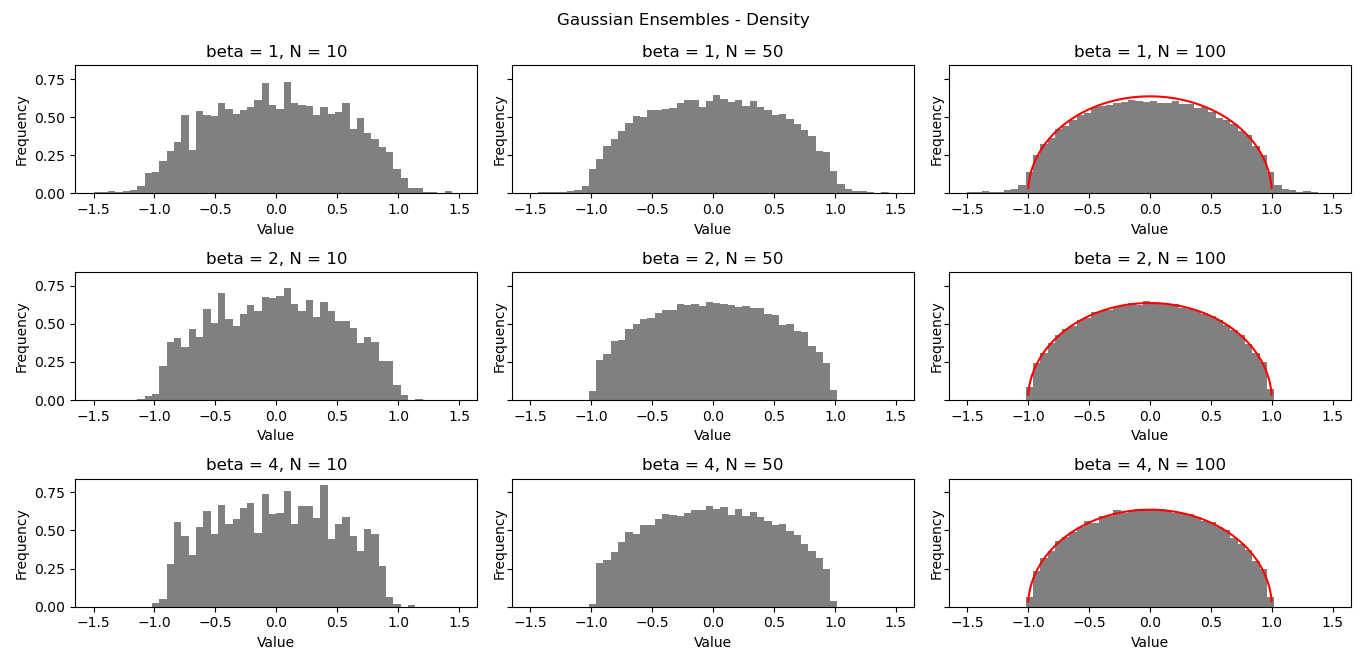
\includegraphics[scale=0.45]{images/validationArticleAlg}
	\caption{Validação para ensembles clássicos, utilizamos $200000$ passos registrando a cada $500$ a partir da metade dos passos. $\Delta t = 0.1$, $\gamma = 1$, $\alpha = 1.0$. Para replicar a semente foi $987991650$.}
\end{figure}

\subsection{Outras distribuições}

\subsubsection{Potencial Quártico}

\begin{center}
	\begin{figure}
		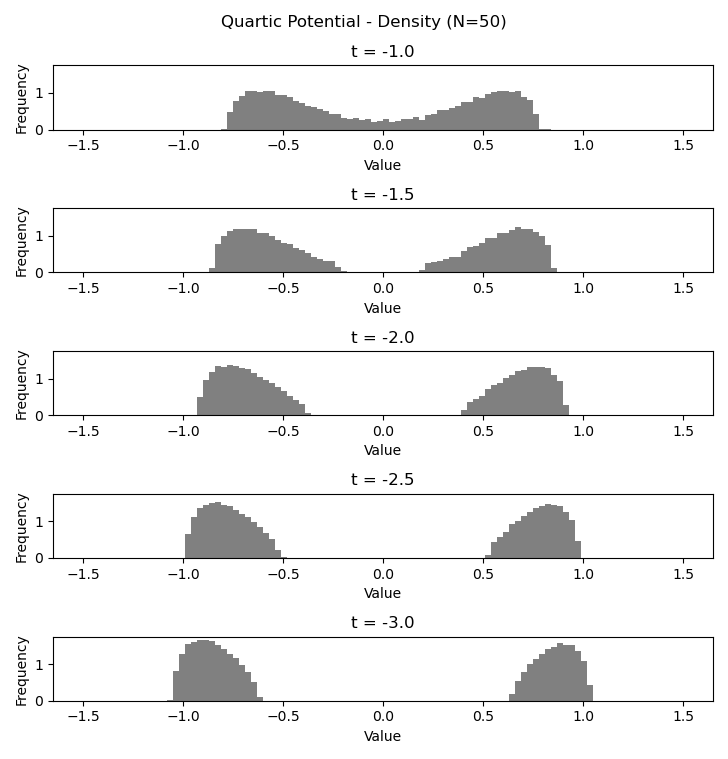
\includegraphics[scale=0.9]{images/validationArticleQuartic}
		\caption{Validação para potencial quártico, $V(x) = \frac{1}{4} x^4 + \frac{t}{2} x^2$. Utilizamos $1000000$ passos registrando a cada $500$ a partir da metade dos passos. $\Delta t = 0.1$, $\gamma = 10$, $\alpha = 0.1$. Para replicar a semente foi $987991650$.}
	\end{figure}
\end{center}

\subsubsection{Potencial Mônico}

\begin{center}
	\begin{figure}
		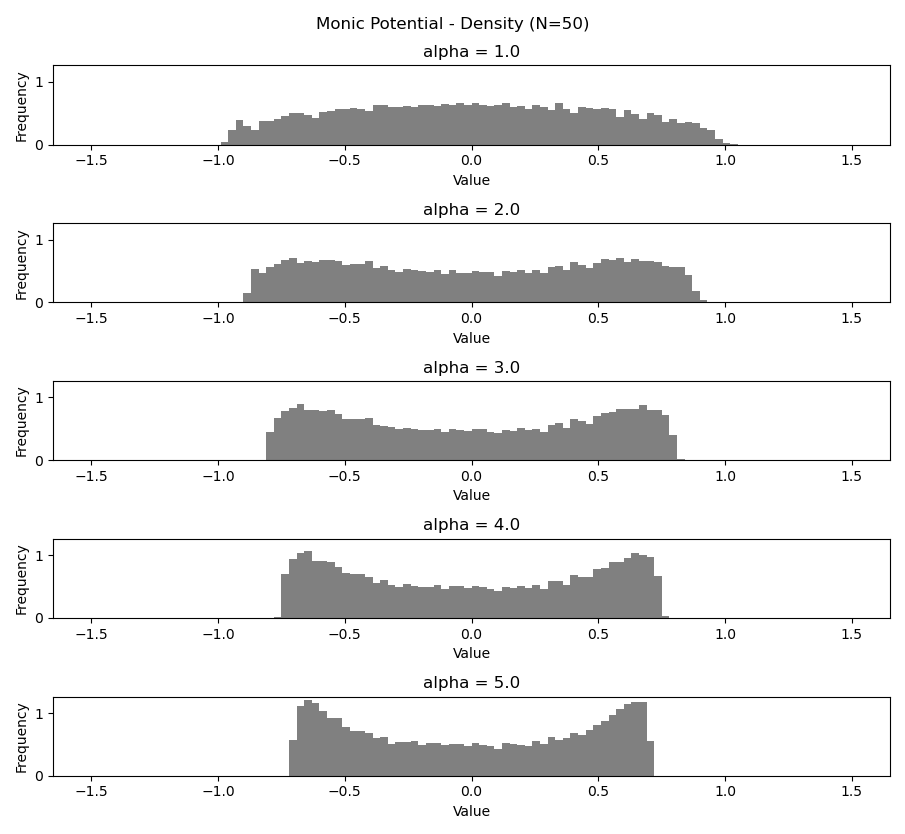
\includegraphics[scale=1]{images/validationArticleMonic}
		\caption{Validação para potencial mônico, $V(x) = \frac{t}{2 \alpha} x^{2\alpha}$. Utilizamos $1000000$ passos registrando a cada $500$ a partir da metade dos passos. $t = 1$, $\Delta t = 0.1$, $\gamma = 10$, $\alpha = 0.1$. Para replicar a semente foi $987991650$.}
	\end{figure}
\end{center}

\subsection{Paralelização}



\bibliography{references}{}
\bibliographystyle{plain}

\appendix

\chapter{Algoritmo Artigo}
\label{apdx: codeArtAlg}
\inputminted[
frame=lines,
framesep=2mm,
baselinestretch=1.2,
bgcolor=white,
fontsize=\footnotesize,
linenos]{FORTRAN}{./code/HKMC.f}


\chapter{Transformação Legendre}
\label{apdx: legendre}
Transformações de Legendre tem ampla aplicação e interpretação. Faremos uma breve dissertação de duas possíveis visualizações do processo. 

\section{Tangentes}

Uma primeira interpretação do processo representa uma mudança clara de variável a partir de tangentes de uma função de concavidade bem definida. Faremos 

\[
	y = f(x) \mapsto \psi(\rho) = f(x(\rho)) - \rho x(\rho)
\]

onde 

\[
	\rho \equiv \frac{y - f(x(\rho))}{x - x(\rho)} = \frac{\psi(\rho) - f(x(\rho))}{0 - x(\rho)}
\]


Que podemos visualizar

\begin{center}
	\begin{tikzpicture}[declare function={f(\x)=0.6*\x*\x - 5*\x + 13;}]
		\draw[help lines, color=gray!30, dashed] (-1,-0.9) grid (5.9,4.9);
		\draw[->,thick] (-1,0)--(6,0) node[right]{$x$};
		\draw[->,thick] (0,-1)--(0,5) node[above]{$y$};
		
		\draw[scale=0.5, domain=1:7.3, smooth, variable=\x, blue] plot ({\x}, {f(\x)});
		\draw (0,0.5) -- (2.5,1.4);
		\filldraw[black] (0,0.5) circle (2pt) node[anchor=east]{$\psi(\rho)$};
		\draw[gray, dash dot] (0,1.3) -- (2.3,1.3);
		\filldraw[black] (0,1.3) circle (2pt) node[anchor=east]{$f(x(\rho))$};
		\draw[gray, dash dot] (2.3,0) -- (2.3,1.3);
		\filldraw[black] (2.3,0) circle (2pt) node[anchor=north]{$x(\rho)$};
	\end{tikzpicture}
\end{center}

De forma que a transformada é criada pela projeção desta tangente no eixo x=0.


\section{Otimização}
Outra forma de visualizar a transformada é por um problema mais conveniente de otimização. Definiremos

\[
	\psi(\rho) = \max_x[\rho x - f(x)]
\]

Onde teremos

\begin{center}
	\begin{tikzpicture}[declare function={f(\x)=0.2*\x*\x;}]
		\draw[help lines, color=gray!30, dashed] (-1,-0.9) grid (5.0,4);
		\draw[->,thick] (-1,0)--(5,0) node[right]{$x$};
		\draw[->,thick] (0,-1)--(0,4) node[above]{$y$};
		
		\draw[scale=0.5, domain=0:6, smooth, variable=\x, blue] plot ({\x}, {f(\x)});
		\draw (0,0) -- (4,3);
		\node[above left] at (3.0,0.5) {\footnotesize $y=f(x)$};
		\node[below right] at (0.3,1.5) {\footnotesize $y=\rho x$};
	\end{tikzpicture}
\end{center}

Se definirmos 

\[
	g(x) = \rho x - f(x)
\]

Minimizaremos $g(x)$ e teremos a condição $f'(x^*) = \rho$. Ou seja

\[
	f'(x(\rho))=\rho \implies \max_x[\rho x - f(x)] = \rho x(\rho) - f(x(\rho))
\]

Que é equivalente à dizer

\[
\psi(\rho) = \min_x[f(x) - \rho x] = f(x(\rho)) - \rho x(\rho)
\]


\chapter{Soma Assintóticas}
\label{apdx: somaassin}
Existe uma aproximação a se fazer no logaritmo de somas assintóticas que pode ser de interesse. Assuma

\[
	S = \sum_{i=1}^{M} a_i
\]  

Se $a_i(N) \sim e^{\phi_i N}$ ou $\log{(a_i)} \approx \phi_i N$, podemos afirmar

\[
	\log{(S)} \sim \log{(a_{max})}
\]

Para demonstrar isso, notamos

\[
	a_{max} < S < M_{a_max}
\]
\[
	\frac{\log{(a_{max})}}{N} < \frac{\log{S}}{N} < \frac{\log{(a_{max})}}{N} + \frac{\log{M}}{N}
\]

Ou seja, desde que $\frac{\log{M}}{N} \rightarrow 0$. Isto ocorrerá desde que $M$ seja sub-exponencial. Contudo \textbf{NOTE} que dizer

\[
	\log{(n!)} \sim n \log{n} - n
\]

Não implica que

\[
	n! \sim ! \left( \frac{n}{e}\right)^n 
\]

Em algumas situações é possível afirmar contudo

\[
	n! \sim \left( \frac{n}{e}\right)^n \sqrt{2\pi n}
\]

\chapter{Det Vandermonde}
\label{apdx: vandermonde}
A formulação nos diz

\begin{equation}
	|V| = \prod_{1\leq i < j \leq n} (\alpha_j - \alpha_i)
\end{equation}

Note que podemos iniciar com uma matriz $n\cdot n$. Seja $c_i$ a coluna $i$, multiplicamos a coluna $c_i$ por $-\alpha_1$ e somamos com a coluna $c_{i+1}$

\[
V = 
\begin{bmatrix}
	1 & \alpha_1 & \alpha_1^2 & \dots & \alpha_1^{n-1} \\
	1 & \alpha_2 & \alpha_2^2 & \dots & \alpha_2^{n-1} \\
	1 & \alpha_3 & \alpha_3^3 & \dots & \alpha_3^{n-1} \\
	\vdots & \vdots & \vdots & \ddots & \vdots \\
	1 & \alpha_n & \alpha_n^2 & \dots & \alpha_n^{n-1}
\end{bmatrix}
=
\begin{bmatrix}
	1 & 0 & 0 & \dots & 0 \\
	1 & \alpha_2 - \alpha_1 & \alpha_2(\alpha_2 - \alpha_1) & \dots & \alpha_2^{n-2}(\alpha_2 - \alpha_1) \\
	1 & \alpha_3 - \alpha_1& \alpha_3(\alpha_3 - \alpha_1) & \dots & \alpha_3^{n-2} (\alpha_3 - \alpha_1)\\
	\vdots & \vdots & \vdots & \ddots & \vdots \\
	1 & \alpha_n- \alpha_1 & \alpha_n(\alpha_n - \alpha_1) & \dots & \alpha_n^{n-2}(\alpha_n - \alpha_1)
\end{bmatrix}
\]

Utilizando do Teorema de Laplace, o determinante vai ser definido simplesmente por

\[
|V| =
	\begin{vmatrix}
		\alpha_2 - \alpha_1 & \alpha_2(\alpha_2 - \alpha_1) & \dots & \alpha_2^{n-2}(\alpha_2 - \alpha_1) \\
		\alpha_3 - \alpha_1& \alpha_3(\alpha_3 - \alpha_1) & \dots & \alpha_3^{n-2} (\alpha_3 - \alpha_1)\\
		\vdots & \vdots & \ddots & \vdots \\
		\alpha_n- \alpha_1 & \alpha_n(\alpha_n - \alpha_1) & \dots & \alpha_n^{n-2}(\alpha_n - \alpha_1)
	\end{vmatrix}
\]

De onde é claro, podemos fatorar os coeficientes e ter

\[
|V| = (\alpha_2 - \alpha_1)(\alpha_3 - \alpha_1)\dots(\alpha_n - \alpha_1)
\begin{vmatrix}
	1 & \alpha_2 & \alpha_2^2 & \dots & \alpha_2^{n-2} \\
	1 & \alpha_3 & \alpha_3^2 & \dots & \alpha_3^{n-2} \\
	1 & \alpha_4 & \alpha_4^3 & \dots & \alpha_4^{n-2} \\
	\vdots & \vdots & \vdots & \ddots & \vdots \\
	1 & \alpha_n & \alpha_n^2 & \dots & \alpha_n^{n-2}
\end{vmatrix}
\]

E assim por diante.


\end{document}          
